\chapter{Where? Dark Matter distribution in the Galaxy and the Universe}\label{chapter:distribution}


As discussed in chapter~\ref{sec:evidences}, the average DM density in the Universe is nonzero, see eq.~(\ref{eq:OmegaDMh2}). 
However, there is much more to DM than just this average value. 
Because of structure formation, the distribution of DM in specific systems differs significantly from the average cosmological value.
In particular, in order to interpret the results of direct and indirect DM detection searches (discussed in chapters~\ref{chapter:direct} and~\ref{chapter:indirect}) one needs the DM density distribution, $\rho(\vec x)$, and the DM speed distribution, $f(\vec{x},\vec{v})$, in the Milky Way, as well as in other galaxies and in a variety of other astrophysical systems.
Presently, only educated guesses are available for these quantities, with significant uncertainties. 
In this chapter we discuss the methods with which such guesses are derived, and their results.
We start with two general statements, which are simple, yet at the same time also quite powerful:
 \begin{itemize}
\item[$\circ$] DM tends to be  {\bf roughly spherically distributed} in gravitationally bound systems. 
The initial conditions in structure formation generally predict nearly spherical distributions. 
Normal baryonic matter then collapses in the gravitational well, during which it dissipates energy and cools down, 
resulting in the spinning disks exhibited by many galaxies (see section~\ref{sec:asphericalcow}). 
Unless DM has similarly large scattering cross sections, it has
negligible interactions and thereby negligible dissipation. 
Neglecting the gravitational effects of visible matter, DM therefore conserves a spherical distribution,
so that one can reasonably assume that the DM density  $\rho(r)$ in  astrophysical systems is, to a good approximation, a function of only the radial coordinate $r$. Deviations from this rough approximation are discussed in detail in section \ref{sec:asphericalcow}.

\item[$\circ$] DM is {\bf non-relativistic} in most systems of interest.\footnote{A notable exception are DM particles in a close proximity of a  dense massive body such as a neutron star. In such cases DM particles acquire relativistic speeds and can even transfer their large kinetic energy to the star, see, e.g.,~section \ref{sec:CaptureNS}.} For instance, DM particles bound to our galaxy must have a velocity below the escape velocity, $v_{\rm esc} \approx 500\,{\rm km/s}$. 
Similar considerations hold for other systems such as dwarf galaxies, galaxy clusters, etc, with the appropriate $v_{\rm esc}$.
\end{itemize}
Going beyond the above general statements, 
 $\rho(r)$ and $f(v)$ for any given system could in principle be determined in three conceptually independent ways: 
{A)} {\bf observationally}, by precisely tracing stellar kinematics in a galaxy (or galactic kinematics in a cluster), inferring the underlying gravitational potential, and thereby the density and velocity distribution of matter responsible for the observed motion of tracers; 
{B)} via {\bf theoretical methods}, describing (semi-)analytically the process of gravitational collapse and its end result; 
{C)} with {\bf ${\bm N}$-body numerical simulations}. 

In practice, A) is too imprecise to provide the full $\rho(r)$,
but it helps in determining the local DM density;
B) faces formal and technical difficulties, due to the non-linear nature of the problem and due to the presence of baryonic physics, yet it provides valuable insights into the complex processes involved.
Therefore, the current most popular approach relies mostly on C), with an admixture of other strategies. Usually, this is a two step procedure:
 \begin{enumerate}
\item Guess the functional forms of $\rho(r)$ and $f(v)$ in terms of a minimal number of free parameters, on the basis of (most often) simulations, or theory, or observations.
\item Determine the free parameters in terms of solid observations of DM in our Galaxy, or in other galaxies.
\end{enumerate}
We will present the results of this procedure in section~\ref{sec:DMdistribution} and \ref{sec:DMv} for the density and speed distributions respectively. 
Finally, in section~\ref{sec:asphericalcow} we discuss how things can be further refined, going beyond the `dark spherical cow' limit.
Before doing that, however, it is worth elaborating on the three methods mentioned above. 

 
\section{Methods to determine the DM distributions} 
 
\subsection{Observations}\label{sec:rho_from_obs}
As discussed in section~\ref{sec:rotatiocurves}, the basic observation that the galactic rotation curves flatten, allows to infer $\rho(r) \propto 1/r^2$ at larger radii $r$, where DM dominates.
One can use the same idea to try to extract  $\rho(r)$ also at smaller $r$:
objects in circular orbits around the galactic center are essentially tracers of the total gravitational potential, hence of the distribution of matter. The mismatch between the rotation curve obtained with such tracers and the one expected from the visible matter in the galaxy\footnote{Here, `galaxy' refers to both the Milky Way, as well as to any other galaxy, including the satellites of the Milky Way, for which one is trying to determine the DM distribution.} must be accounted for by Dark Matter.
The DM density distribution can thus be obtained by fitting an appropriately parametrized function to the total rotation curve \cite{rhoDM_observations}. This is often referred to as the {\em global method} to determine the DM distribution (as opposed to the {\em local} method, discussed below, which is less ambitious, and only aims to determine the DM density at the location of the solar system, and about 1 kpc around it). 


The method is conceptually simple. To obtain the predictions for the rotation curves, the Poisson equation for the Newton potential $\phi$, $\nabla^2\phi = 4\pi G \rho$, is first solved assuming as a source only the observed mass distributions due to baryons in the stars
and from those in the inter-stellar gas,
$\rho=\rho_b=\rho_{\rm star}+\rho_{\rm gas}$, taking into account their
approximate cylindrical (rather than spherical) geometry $r,z,\theta$.
The Newton's equation for a test mass in a gravitational field, $v^2/r = -\partial \phi/\partial r$, 
then predicts the rotation velocity $v(r)=(v^2_{\rm star} + v^2_{\rm gas})^{1/2}$  in the galactic plane, at $z=0$,
where these are measured.\footnote{The velocities orthogonal to the galactic plane and the radial velocities
provide extra information, in principle. In practice, however,  they are not measured well enough.}
Comparison with data for $v(r)$ shows that an extra `dark' contribution is needed in order to reproduce the observations,
\beq
\label{eq:sum:v:squares}
v^2 = v^2_{\rm star} + v^2_{\rm gas} + v^2_{\rm dark},
\eeq
which then allows to determine the DM contribution by subtracting the predictions from observations.


\smallskip

However, a number of difficulties arise. First, stellar kinematical data still carry significant uncertainties, both intrinsic to the measurements and due to their interpretation (also in the Milky Way, related, e.g., to the knowledge of the precise distance of the Sun from the galactic center and of the Sun's circular velocity). 
Second, the results of the mismatch fit, mentioned above, depends crucially on what is being assumed for the visible component of the galaxy.   More precisely, one has to design a {\it  model of the galaxy} as a system composed of a bulge, a possible bar, a disk, a gas halo, and possibly even a smaller disk at the core of the bulge\ldots, each of these appropriately modeled using several observation-based configurations. 
The gas density is extracted, e.g.,~from the 21 cm maps, while the stellar models are needed to convert observed luminosity into mass density.
The uncertainties on these {\em baryonic morphologies} are still sizeable, despite the recent improvements due to the fact that data mostly based on optical observations are now being replaced by the near-IR data, which need only minor modeling corrections.
Finally, since the baryonic matter dominates the gravitational potential in the inner few kpc of galaxies (the inner $\sim$5 kpc for the Milky Way), the contribution of DM is intrinsically very difficult to determine in that region. 

\medskip

In practice, therefore, observational methods are sufficient to affirm the presence of DM in galaxies and to get a rough idea of its large scale distribution, but are at present not sufficient for more precise determinations. 




\subsection{Gravitational collapse of collision-less DM} 
\label{sec:rho_from_analytic}
\index{Gravitational collapse}
\index{Virialization}
The formation of a Dark Matter galactic halo is a conceptually well defined theoretical problem: 
start from a roughly spherical slight over-density made of collision-less and dissipation-less bodies, and let it evolve under gravity. 
The system starts collapsing under its own weight (and at some point the inhomogeneity grows beyond the computable linear approximation) but {\em the collapse self-limits without reaching a point with infinite density}.
This happens because DM is collision-less and cannot dissipate energy, so during the collapse its gravitational potential energy has to be converted into kinetic energy of the DM particles involved. 
The sphere therefore eventually relaxes to a self-gravitating quasi-static structure supported by random motions of DM particles. 
The whole process is referred to as {\em virialization} and the resulting system is {\em virialized}, i.e.,~its energy is distributed between the potential energy, $V$, and kinetic energy, $K$, according to the virial theorem $\langle K\rangle = -\frac{1}{2}\langle{V}\rangle$ (already mentioned in section~\ref{sec:evidencesmedi})~\cite{books_galaxy_formation}. 

\medskip




The virial theorem provides enough information to estimate the typical scales involved.
For simplicity, we consider a spherical DM over-density with homogeneous density of total mass $\Mcal _{\rm tot}$
(ellipsoidal collapse models with non-constant density are also considered in the literature).
The main phases, discussed below, are illustrated in fig.\fig{SphericalCollapse}.
We define $\rho_{\rm ta}$ as the homogeneous density  at the instant of {\em turnaround}, 
i.e.,~at the moment at which the over-density 
stops following the expansion caused by the Big Bang, stalls, and turns around to start collapsing into a gravitationally bound object. This marks
 the onset of  structure formation. 
Since DM is stalling, its kinetic energy $K_{\rm ta}$ vanishes, and thus its total energy $E_{\rm ta} = K_{\rm ta}+ V_{\rm ta} $ is entirely due to its gravitational
potential energy 
\beq V_{\rm ta} = -G \int_0^{r_{\rm ta}} \left(\frac{4\pi r^3}{3} \,  \rho_{\rm in}\right) \frac{4\pi r^2  \, dr\,  \rho_{\rm ta}}{r} 
= - \frac{3}{5}\frac{G \Mcal _{\rm tot}^2}{r_{\rm ta}},\eeq 
where $r_{\rm ta}$ is the size of the sphere at turnaround, and 
$\rho_{\rm in}$ is the density inside the sphere (in our approximation taken equal to $\rho_{\rm ta}$).

If spherical symmetry were absolutely exact, i.e., if all DM particles were following a perfectly radial trajectory, the collapse would have proceeded toward infinite density, forming a black hole.
In reality, the system keeps sphericity only on average and reaches a finite density thanks to the chaotic motion of DM particles, interacting only via gravity.
After this {\em virialization} process the energy is distributed between the kinetic and potential energy, such that $E_{\rm vir} = K_{\rm vir} + V_{\rm vir} = V_{\rm vir}/2$, where the last equality follows from the virial theorem. Since virialization conserves the total energy, the potential energy $V_{\rm vir} = -3 G \Mcal _{\rm tot}^2/5r_{\rm vir}$ 
(we still approximate the density as constant, $\rho_{\rm vir} = \Mcal _{\rm tot}/(\frac43\pi r_{\rm vir}^3)$,
where now $r_{\rm vir}$ is the radius of the virialized halo) therefore implies $r_{\rm vir} = r_{\rm ta}/2$. That is, 
the collapse results in a relaxed halo half the size of the turn-around bubble, 
with an order of magnitude higher density, $\rho_{\rm vir}=8\rho_{\rm ta}$.\footnote{
This means that the collapse of collision-less DM does {\em not} form black holes.
The situation is strikingly different for normal matter. 
Since normal matter has large scattering cross sections, it is opaque to photons, 
so that these are emitted into surroundings only by surfaces of compact objects and not by the whole volumes. 
A non-spherical collapse of a large over-density of normal
matter  tends to fragment, thereby  forming many stars, rather than one big object.
Stars can then evolve into stellar-mass black holes. 
How the super-massive black holes form is an area of active research, 
with one possibility that they form from accretion of dust, gas, as well as stars and stellar-mass black holes.
}
The mean square speed of virialized particles is $\langle v^2 \rangle = 2 K_{\rm vir}/\Mcal _{\rm tot}= |V_{\rm vir}|/\Mcal _{\rm tot} = 3G \Mcal _{\rm tot}/5r_{\rm vir}$. 
Solving Newton equations for a homogeneous density in an expanding matter-dominated universe
shows that the average density of the formed halo $\rho_{\rm vir}$  is roughly $ 200$ times the 
surrounding cosmological density 
\beq\label{eq:rhovir}
\bar \rho = \frac{3 H^2}{8 \pi G} = \frac{1}{6 \pi \, G \, t_{\rm vir}^2},\eeq
where $t_{\rm vir}$ is the time marking the end of virialization~\cite{books_galaxy_formation}
(here we used eq.~(\ref{eq:rhocrit}) and eq.~(\ref{eq:aandHinMDRD}) for matter domination). 
Quite often the {\em virial radius} is thus defined as the radius within which the average density of the halo is 200 times larger than the cosmological density,  
and is denoted as $r_{200}$. 
The mass inside $r_{200}$ is taken as a measure of the total mass of the halo.
The reality, at least as seen in numerical simulations, is more involved, but orders of magnitude are correct.



\begin{figure}[t]
\begin{center}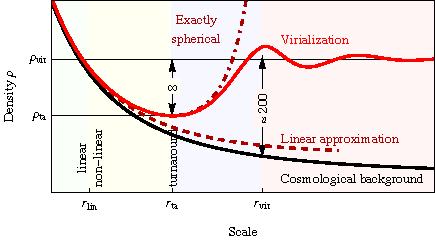
\includegraphics[width=0.6\textwidth]{figs/SphericalCollapseCartoon}\end{center}
\caption[Gravitational collapse]{\em\label{fig:SphericalCollapse} Qualitative illustration of the main phases of a nearly-spherical {\bfseries gravitational collapse}.  The dot-dashed curve shows the result assuming an unrealistic exact spherical symmetry;
the continuous red curve shows the realistic result;
the dashed curve shows the result within linear approximation,
which remains close to the cosmological background (bottom black curve).
}
\end{figure}


\medskip


Besides its global properties, one can gain a slightly more refined understanding of the final DM halo (in particular its density and speed distributions, in which we are interested here) by following analytically the collapse and paying particular attention to the {\em relaxation} mechanisms.  
There are several such dynamical processes at play, driving the system toward an equilibrium configuration~\cite{books_galaxy_formation}. 
The important mechanism for collision-less DM particles is the so called {\em violent relaxation}~\cite{Lynden-Bell1967}:
the energy of an individual DM particle changes with time due to the fact that the gravitational potential in which these are immersed (generated by the ensemble of DM particles themselves) also changes with time, because of the ongoing collapse. 
This mechanism works in an efficient way on the short timescale of the collapse, hence the name `violent'. 
The total energy of a given DM particle divided by its mass, 
$\varepsilon =  v^2/2 + \varphi$, varies as
$d\varepsilon/dt = \partial \varphi/\partial t$, if the gravitational potential is time dependent.
The last relation is straightforward to verify,
\begin{equation*}
\frac{d \varepsilon}{dt} = \frac{\partial \varepsilon}{\partial \vec v} \cdot \frac{ d \vec v }{dt} + \frac{\partial \varepsilon}{\partial \varphi} \frac{d \varphi}{d t} = 
\vec v \cdot (- \vec\nabla \varphi )+ 1\left(\frac{\partial \varphi}{\partial t} + \vec v \cdot \vec\nabla \varphi \right)= \frac{\partial \varphi}{\partial t},
\end{equation*}
where the equalities follow trivially from the chain rule, the definition of $\varepsilon$ and from $d \vec v/dt = -\vec\nabla \varphi$, 
which is the Newton's law, $\vec a = \vec F/m$, for the case of just gravitational interactions. 


Whether the particle gains or looses energy is a complex question.
One can qualitatively figure out what is going on by thinking of a DM particle that starts collapsing from the outskirts of the halo (which itself will first collapse and then expand, until the particles virialize). During the infall, the DM particle will dive into a deep potential due to the collapsing halo and gain kinetic energy. 
After crossing the center (unscathed, because of its collision-less nature), it will climb out of a shallower potential, because its fellow DM particles are dispersing, and will therefore spend less than the previously acquired kinetic energy, resulting in a net energy gain. The opposite happens for particles that start from inner locations. For instance, a particle at rest in the center does not move, while as the protohalo collapses, the potential at its center becomes deeper. In general, the gain or loss of energy of a single particle depends on its initial position and initial speed, as well as on the distribution of all other DM, in a complex way~\cite{books_galaxy_formation,Lynden-Bell1967}.

\smallskip

The whole process effectively amounts to 
DM particles undergoing many  gravitational interactions.
As a consequence, their final velocities are given by a sum of many random contributions.
Due to the Central Limit Theorem their energy distribution will tend toward 
a Gaussian:
\beq\label{eq:DMdensGauss}
f(\varepsilon) = \frac{n_0}{(2\pi\sigma^2)^{3/2}} \ e^{-\varepsilon/\sigma^2}, 
\eeq
where the peculiar form of the normalization factor multiplying the exponential will be clear soon. 
The exponent is $\varepsilon = \frac12 \vec v^2 + \varphi$, from which it immediately  follows that the energy distribution $f(\epsilon)$ can be interpreted as the distribution of DM speeds, $f(v)$, taking the Maxwell-Boltzmann form
\beq
f(v) \propto e^{-v^2/2 \sigma^2}.
\eeq
The uniform `temperature' (related to velocity dispersion $\sigma$) is for a fully virialized halo given by its total mass. 

\index{Eddington inversion}
To show that, we move next to the discussion of the DM density distribution, $\rho(r)$. For spherically symmetric systems there is a unique correspondence between $f(v)$ and $\rho(r)$ (this general relation is known as the {\it Eddington's formula}, and the art of deriving $\rho(r)$ from $f(v)$ as the {\it Eddington inversion}). It can be derived 
by first 
integrating $f(\varepsilon)$ over all velocities,\footnote{More precisely, 
what we are actually dealing with is the distribution function $f(\vec x,\vec v, t)$, defined such that $f(\vec x,\vec v, t) \, d^3\vec x \, d^3\vec v$ is the probability at time $t$ of finding a particle in the $d^3\vec x\,  d^3\vec v$ phase space volume centered at $\vec x, \vec v$.
For a spherical steady-state system it can be shown that $f$ depends on $\vec x, \vec v$ only through the total energy, which is an integral of motion ($f$ is said to be {\it ergodic}). That is why by integrating $f(\varepsilon)$ over all velocities one obtains the spatial distribution of DM particles, i.e.,~their number density (the use of $n_0$ in the normalization factor in \eqref{eq:DMdensGauss} was already the first hint for this).  Multiplying it by the DM mass $M$ one then obtains the mass density $\rho$. 
For more details see, e.g.,\ chapter 4 in Binney \& Tremaine~\cite{books_galaxy_formation}.
}
which then gives an implicit expression for the DM density distribution \index{Isothermal sphere}
\beq
\label{eq:rho_isothermal_almostthere}
\rho = M \int_0^\infty dv \, 4\pi v^2 f(\epsilon) = M \int_0^\infty dv \, 4\pi v^2 \ \frac{n_0}{(2\pi\sigma^2)^{3/2}} \ e^{-(v^2/2+\varphi)/\sigma^2} = \rho_0 \ e^{-\varphi/\sigma^2},
\eeq
with $\rho_0 = M n_0$. 
Eq.~(\ref{eq:rho_isothermal_almostthere}) gives the gravitational potential in terms of $\rho$.
Inserting this expression into Poisson's equation, $\nabla^2 \varphi = 4\pi G  \, \rho$, written in spherical coordinates, leads to
\beq
\frac{d}{dr}\left( r^2 \frac{d}{dr} \ln \rho \right) = -\frac{4\pi \, G} {\sigma^2} r^2 \rho.
\eeq
The solution is 
\beq\label{eq:isothermalsphere}
\rho(r) = \frac{\sigma^2}{2\pi G} \frac{1}{r^2}.
\eeq
This distribution is the {\em singular isothermal sphere}. The name comes from the fact that this is the same equilibrium configuration, characterized by a single $r$ independent temperature $T$, to which an ideal gas is driven by collisions and interactions. 
The role of `collisions and interactions'  is played  here by the gravitational scatterings between DM particles and the whole halo, with the effective cross-section given by 
\beq 
\sigma_{\rm grav} = \frac{G \, M \Mcal _{\rm tot}}{r^2 v^{4}}.
\eeq
In our case, the quantity that is constant with radius is the velocity dispersion $\sigma$: the correspondence with the case of an ideal gas is achieved if one identifies $\sigma^2 = k_B T/M$, where $k_B$ is the Boltzmann constant. 


\medskip

In summary, 
the classical theory of collapse of isolated, spherical, collision-less and dissipation-less systems 
predicts equilibrium DM halos that are singular isothermal spheres with exactly Maxwell-Boltzmann speed distributions. This is often called the {\em Standard Halo Model} (SHM).

\medskip


In practice, the singular isothermal model is just an idealized approximation. 
First, the resulting rotation curve is exactly flat, \label{vcircisot} $v^2_{\rm circ}(r) = G\Mcal (r)/r = 2\sigma^2$, which is not what realistic measurements show.
Also, its density diverges as $r\to 0$, but this is not a dramatic problem
since the mass enclosed within radius $r$ is finite,
$\Mcal (r) = \int_0^r dr\, 4\pi r^2\,\rho = 2\sigma^2 r/G$.
On the other hand, integrating towards large $r$,
the total mass diverges, which is absurd from the astrophysical point of view: the profile must therefore be amended and truncated at some large radius. More generally, many effects can cause deviations from the simple picture that led to isothermal distribution: i) the collapse process can be incomplete and not reach a full equilibrium state, 
ii) the assumption of spherical symmetry is easily violated by non-radial deformations in the initial conditions, 
iii) the hypothesis that the system is isolated is not valid for halos embedded in the DM cosmic web: inflows, outflows and mergers cannot typically be neglected, etc. 

The Standard Halo Model can be extended to correct for some of these shortcomings, making it more realistic~\cite{books_galaxy_formation,AnalyticalHM}, although often at the price of a more involved analytical treatment (see also the discussion in section \ref{sec:asphericalcow}). 
Given these complexities and the limitations of purely analytical approaches, numerical simulations have increasingly become an important tool to determine the properties of the DM halos.
 We discuss these next.


\begin{figure}[t]
\begin{center}
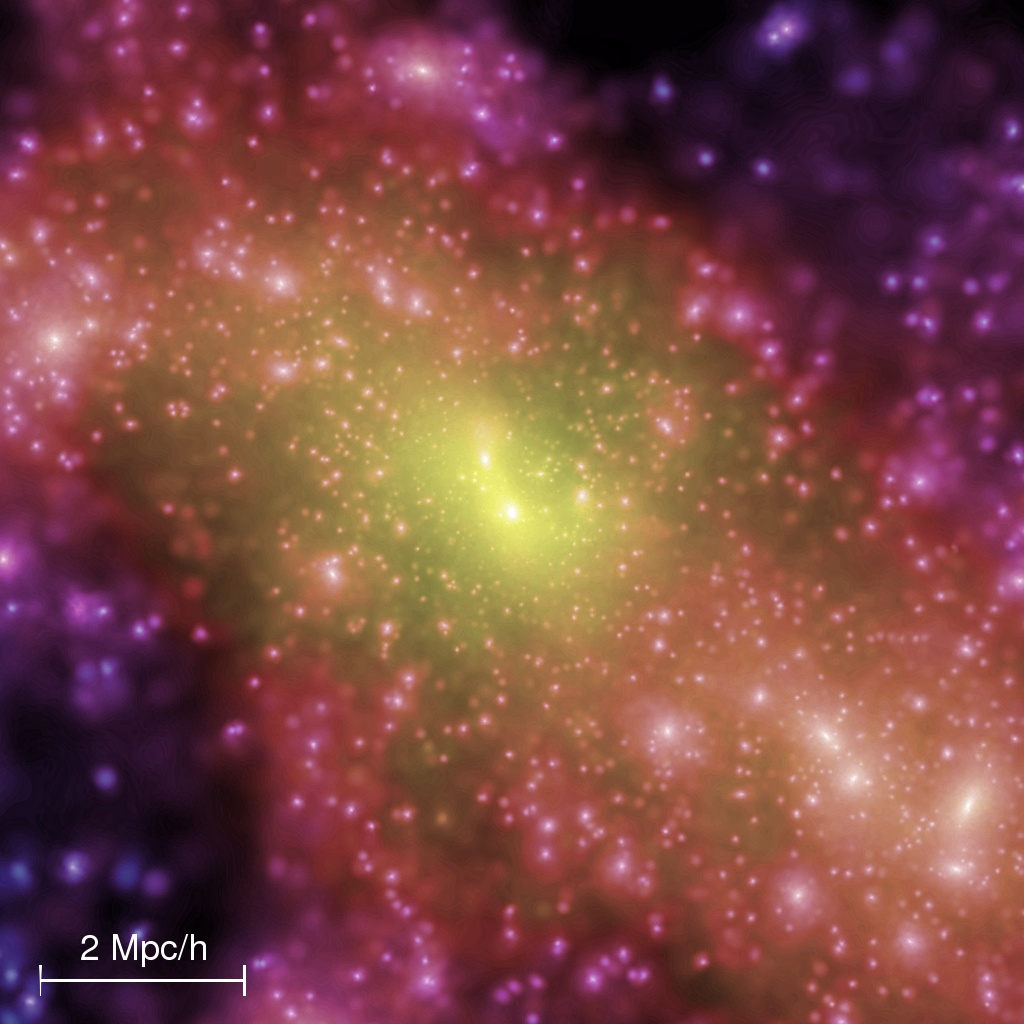
\includegraphics[width=0.45\textwidth]{figs/Millenium_1.jpg} \
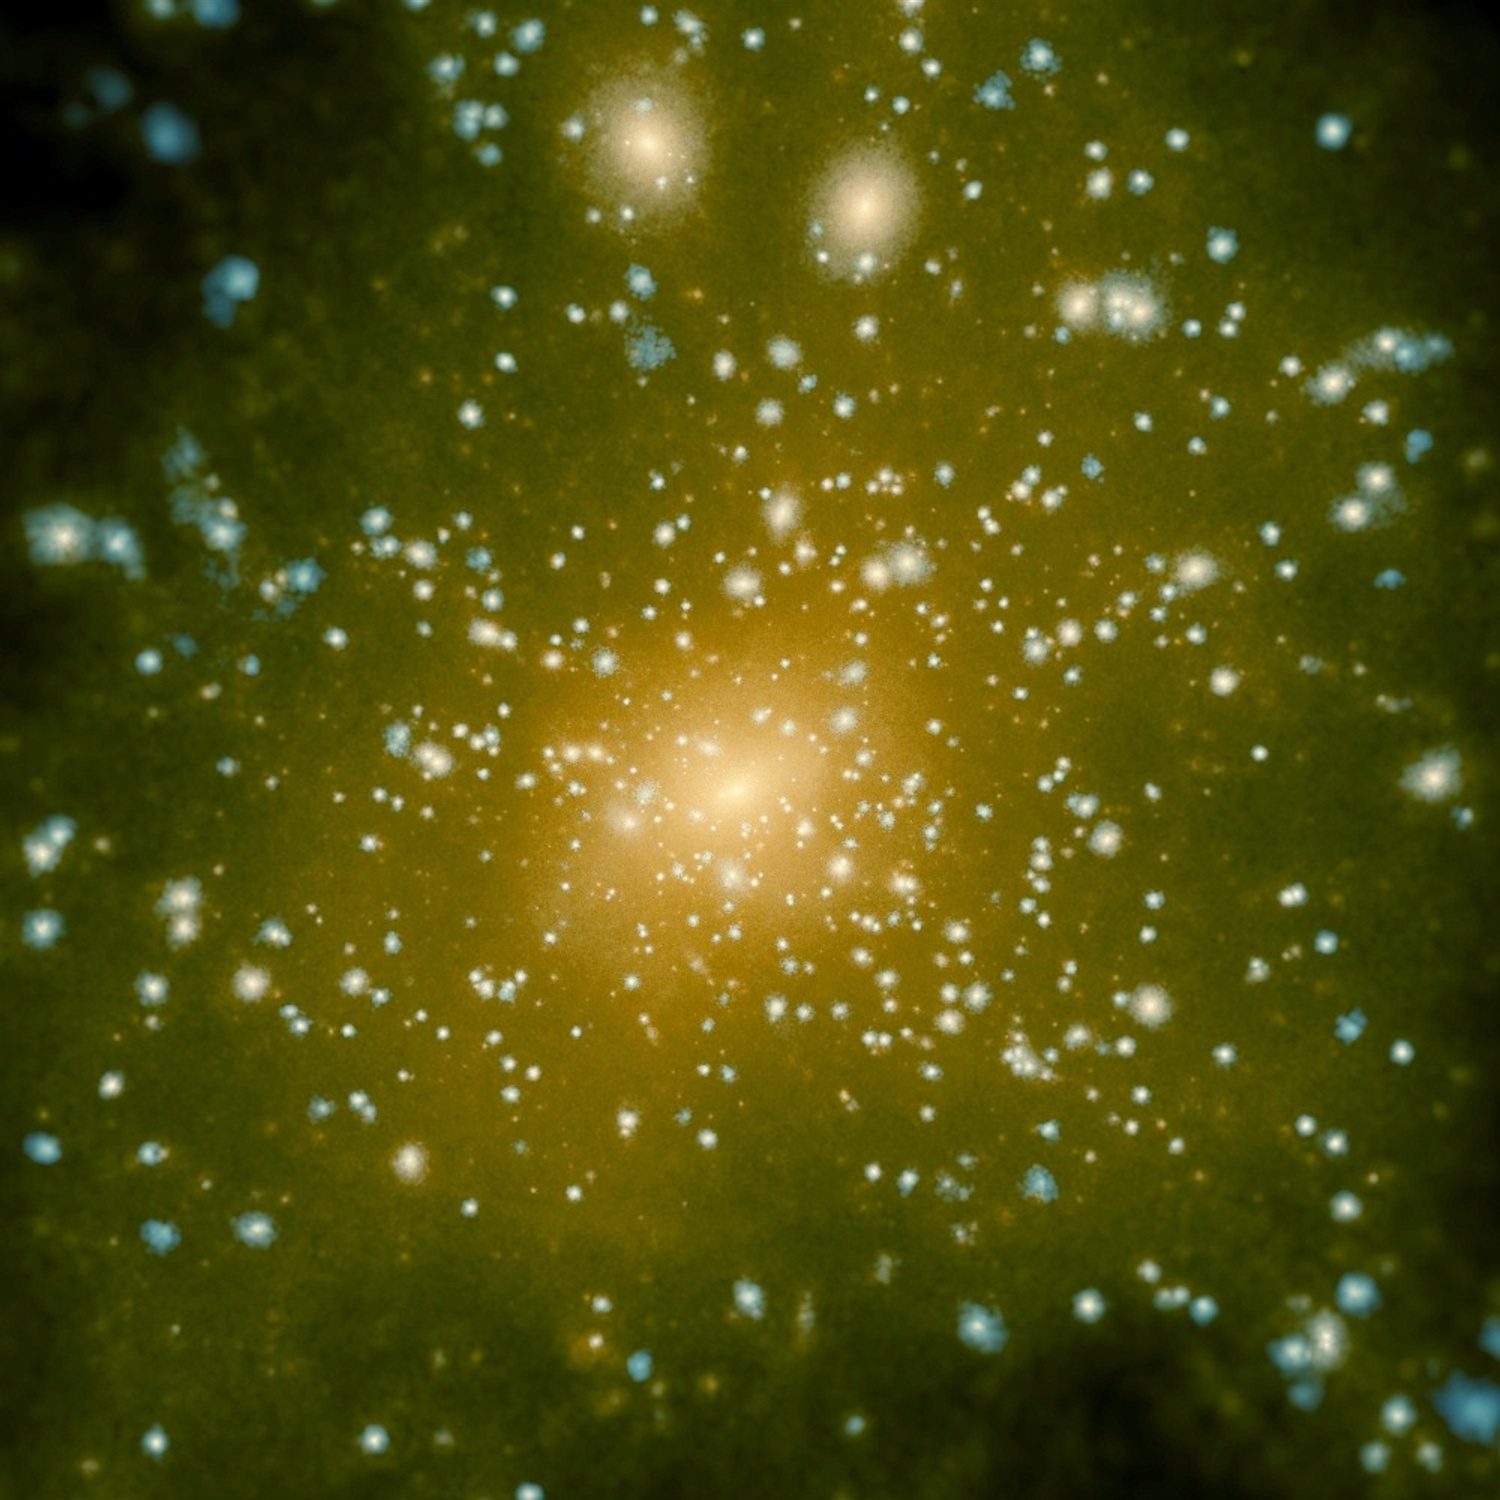
\includegraphics[width=0.45\textwidth]{figs/Millenium_2.jpg}
\end{center}
\caption[DM sub-halos]{\em\label{fig:Sub-halos} {\bfseries Sub-halos}. 
$N$-body simulations find that DM forms roughly spherical halos, which are then surrounded as well as inhabited by many smaller sub-halos. From simulation realized at the \href{https://wwwmpa.mpa-garching.mpg.de/galform/index.shtml}{MPI}, credit: Max-Planck-Institute for Astrophysics.}
\end{figure}


\subsection{Results from $N$-body simulations}\label{sec:resNbody}

Since statistical mechanics does not provide sharp general answers, the gravitational collapse of dark matter is also studied numerically,  using the $N$-body simulations~\cite{Nbody}, which we already introduced in section~\ref{Nbody}. 
While such computer codes do not simulate a specific galaxy 
(we are especially interested in the Milky Way, or local dwarfs), but rather an ensemble of more or less typical galaxies, their results do show that the DM halos density profiles tend to possess some universal features, as summarized below.

\medskip

DM halos are produced with sizes that span all simulated scales:
from cosmological scales around $100$ Mpc down to sub-galactic scales of tens of pc,
ranging about 20 orders of magnitude in the enclosed mass $\Mcal $.
The number of halos, $n$, as a function of their mass scales roughly  as $dn/d\Mcal  \propto 1/\Mcal ^2$, and
will be  discussed analytically in section~\ref{sec:haloMf}.

\smallskip

To a first approximation, luminous matter follows the distribution of the large scale structure,  i.e.,~galaxies form where matter is dense. However, galaxies do not trace {\em exactly} the underlying DM distribution, because galaxy formation proceeds with an efficiency that depends on the halo mass. The relationship between the mean over-density of galaxies $\delta_{\rm gal}$ and the mean overdensity of the total mass $\delta_{\rm tot}$ (dominated by DM) is complicated. Their ratio, the so called {\em bias} $b=\delta_{\rm gal}/\delta_{\rm tot}$, is in general a function of the scale,  the properties of the galaxy in question, and the redshift. Numerical simulations complement the analytical results (as pioneered, e.g., by Kaiser (1984) and Bardeen (1986)~\cite{bias}), 
and show that galaxies preferentially form in halos that are not too small (otherwise supernova feedback hampers the collapse) nor too large (otherwise gas does not cool efficiently enough).

\smallskip

Simulations of cold collision-less DM produce DM halos, which have in general an {\em ellipsoidal shape}, rather than being spherical. 
The non-sphericity is limited, however, and is found to be smaller in simulations that include baryons, as we will discuss in section~\ref{sec:nonSphericalHalo}. 
The standard assumption of sphericity, adopted in most phenomenological studies, is therefore quite reasonable.

\smallskip



\smallskip

The {\bf density profiles} $\rho(r)$ of individual halos, computed from numerical data in spherical approximation, 
tend to follow a universal slope $s(r) \equiv d\ln \rho/d\ln r $ that smoothly changes from $\sim -1$ (in the inner region) to $\sim -3$ (in the outer region).
For comparison, the isothermal sphere, suggested by the analytic considerations in eq.\eq{isothermalsphere}, has $s=-2$. 
The results of simulations can be fitted by functions such as the ones in table~\ref{tab:rhoprofiles}
dubbed `NFW' (from Navarro, Frenk, White; with a slope that changes from $-3$ to $-1$ around the radius $r_s$)
 or `Einasto' (with a slope that equals $-2$ at $r=r_s$ and continuously evolves). 
The  numerical values of DM density profile fit functions for Milky Way will be discussed in section~\ref{sec:MilkyWay}.
The individual gravitationally bound objects can be simulated down to sizes about 3 orders of magnitude smaller than their
virial radius $r_{\rm vir}$
(defined such that the $\rho(r_{\rm vir})$ is 200 times  larger than the mean density,
for  reasons discussed in section \ref{sec:rho_from_analytic}).
The simulations thus cannot resolve a possible core (where the density $\rho$ becomes constant), if it is too small. 
As a rule of thumb, for a galaxy like the Milky Way, the existence of a core with a size below $\approx 1$ kpc 
is compatible with the current simulations. 

\smallskip

\index{Numerical simulations!sub-halos}\index{Sub-halos}
In addition to the primary halo structures, simulations reveal the presence of numerous smaller {\bf sub-halos} (see fig.\fig{Sub-halos})
orbiting within and around main halos. Their number distribution is $dn/d\Mcal  \approxprop 1/\Mcal ^2$, so that
$\Mcal\,  dn/d\ln \Mcal $ is roughly $\Mcal $-independent.
That is, similar amounts of total DM mass are stored within objects for any given decade in mass scale $\Mcal $,
from the biggest formed structures down to the smallest resolved structures, of the order $\Mcal \approx 10^5 \  M_\odot$ \cite{subhaloproperties}.
Additional smaller halos, not yet resolved by the simulations, are expected to exist\footnote{The possible detection of a DM sub-halo with mass of few $10^7\, M_\odot$ in a region of the Milky Way near the Sun is claimed in~\cite{2507.16932}. The authors employed high-precision pulsar timing to reconstruct the accelerations of several pulsars, finding that these accelerations appear to be directed toward a region 
where the observed visible matter alone cannot account for the required gravitational pull.}, as also anticipated by the analytic arguments to be discussed in section~\ref{sec:haloMf}.
Simulations show that these sub-halos possess higher inner DM densities and are, on average, more concentrated than stand-alone halos of the same mass.
In section~\ref{sec:astroboost} we will discuss how the presence of sub-halos boosts the indirect signals of DM annihilations.

Other features of simulated halos seem less universal. 
The concentration parameter of any halo is defined as $c=r_{\rm vir}/r_{-2}$
where $r_{-2}$ is the radius at which the slope reaches $s=-2$ ($r_{-2}=r_s$ in the Einasto parameterisation).
The mass of the smallest halos, called {\bf micro-halos}, 
will be discussed in section~\ref{sec:haloMf}: it depends on DM particle properties
and could, for weak-scale DM, be comparable to Earth's mass, $10^{-6}M_\odot$.
Micro-halos do not form from merging of smaller halos ---
dedicated simulations suggest that they tend to have $c\approx 20-30$~\cite{MinimalHaloMassandFS}.
The concentration parameter $c$ gradually decreases down to $c\sim$ few  for larger objects (galaxies and clusters), 
which formed earlier, when the universe was denser.
Sub-halos inside galactic halos in particular have higher inner DM densities and are, on average, more concentrated than the free-standing halos of the same mass. Moreover, the sub-halos are more concentrated, the closer they are to the center of the host halo~\cite{subhaloproperties}.
Finally, the ratio between the spherically averaged density and the average radial velocity seems to follow a power-law, $\rho/v_r^3 \propto 1/r^{1.875}$.


Simulations have intrinsic limitations: normal matter is only approximatively modeled,
numerical issues remain,  halos selected for more detailed computations are maybe not the typical ones, etc.
Comparing simulations to observations suggest possible discrepancies, discussed in section~\ref{sec:astroanomaly}:
the cusp-core problem, the diversity problem,  and the missing satellite problem.
 
 \smallskip
 
 \index{DM abundance!asphericity}
The results of $N$-body simulations apply to the Milky Way, as long as this is a typical galaxy.
Since we do not know observationally whether or not the Milky Way is surrounded by a halo with an atypically high asphericity, we will later assume that this is not the case, and use an average spherical DM halo to describe the Milky Way.
This may well be an oversimplification: the measured Milky Way stellar velocities indicate that it formed via a relatively recent merging of two big progenitors~\cite{1804.09365,1807.02519}, possibly complicating the DM local distribution.




\section{Dark Matter density distribution}\label{sec:DMdistribution}\index{Density distribution}\index{Einasto profile}\index{NFW profile}\index{Isothermal sphere}\index{Milky Way!DM abundance}

\begin{table}[t]
$$\begin{array}{r|rcl}
\hbox{DM halo} & \multicolumn{3}{c}{\hbox{Functional form}}\\ \hline \rowcolor[rgb]{0.99,0.97,0.97}
{\rm NFW} & \rho_{\rm NFW}(r)  & = & \displaystyle \rho_{s}\frac{r_{s}}{r}\left(1+\frac{r}{r_{s}}\right)^{-2} \\[4mm] \rowcolor[rgb]{0.99,0.97,0.97}
{\rm Generalized \ NFW} &  \rho_{\rm gNFW}(r)  & = & \displaystyle \rho_{s} \left(\frac{r_s}{r}\right)^{\gamma} \left(1+\frac{r}{r_s}\right)^{\gamma-3} \\[4mm] \rowcolor[rgb]{0.99,0.97,0.97}
{\rm Einasto} & \rho_{\rm Ein}(r)  & = & \displaystyle \rho_{s}\exp\left\{-\frac{2}{\alpha_{\rm Ein}}\left[\left(\frac{r}{r_{s}}\right)^{\alpha_{\rm Ein}}-1\right]\right\} \\[4mm] \rowcolor[rgb]{0.97,0.97,0.93}
{\rm Cored} \ {\rm Isothermal} &  \rho_{\rm Iso}(r) & = & \displaystyle \frac{\rho_{s}}{1+\left(r/r_{s}\right)^{2}} \\[4mm] \rowcolor[rgb]{0.97,0.97,0.93}
{\rm Burkert} & \rho_{\rm Bur}(r) & = & \displaystyle  \frac{\rho_{s}}{(1+r/r_{s})(1+ (r/r_{s})^{2})}.
\end{array}
$$
\caption[DM density profiles]{\label{tab:rhoprofiles}\label{eq:profiles}
\em Plausible  spherical density profiles $\rho(r)$ for DM halos in galaxies.}
\end{table}

\setstretch{0.97}
\subsection{Galactic DM density functions}\label{rho(r)}
We review now the galactic DM density distributions $\rho(r)$ often considered as the most plausible in the literature.
All the profiles assume spherical symmetry, with $r$ the radial coordinate measured from the Galactic Center (GC). 
The functions are listed in table~\ref{tab:rhoprofiles}
and plotted in fig.~\ref{fig:DMprofiles} for plausible values of their free parameters $r_s$, $\rho_s$ and $\alpha_{\rm Ein}$.
Some of these functions can be conveniently recast in terms of a collective formula with three parameters $\alpha, \beta, \gamma$ \cite{profilesabc}, also referred to as the `double power-law' formula 
\begin{equation}
\begin{array}{rrclr} 
    {\rm Hernquist} \ \alpha\beta\gamma: & \rho_{\alpha\beta\gamma}(r) & = &  \displaystyle  \frac{\rho_{s}}{(r/r_s)^\gamma \, \Big[1+(r/r_s)^\alpha \Big]^{\frac{\beta-\gamma}{\alpha}} },
    & \quad 
    \begin{minipage}{0.2\textwidth}
\footnotesize{  
\begin{tabular}{rcrc}
 & $\alpha$ & $\beta$ & $\gamma$ \\
  NFW & 1 & 3 & 1 \\
  gNFW & 1 & 3 & $\gamma$ \\
  Cored Iso & 2 & 2 & 0 
 \end{tabular}}.
\end{minipage}
 \end{array}
\label{eq:profilesabc}
\end{equation} 
The parameters $\alpha$, $\beta$, and $\gamma$ control the shape of the DM density profile at different radial distances from the galactic center.
Specifically, $\alpha$ controls the sharpness of the transition between the inner and outer slopes, $\beta$ affects the outer slope, and $\gamma$ determines the inner slope of the profile.
These functions are motivated by the following considerations:
\begin{itemize}
\item[$\triangleright$] 
The Navarro, Frenk and White ({\bf NFW})~\cite{NFW} profile is the most common benchmark choice motivated by the $N$-body simulations.
The density diverges as $r^{-1}$ close to the GC. The version with two parameters fixed, $\alpha =1, \beta =3$, and $\gamma$ taken as a free parameter (in the notation of eq.~(\ref{eq:profilesabc})), is sometimes called the `{\bf generalized NFW (gNFW)}' profile. 
When $\gamma >1$, the slope at the center is steeper than for the standard NFW: in this case the profile is referred to as the `{\bf contracted NFW (cNFW)}'. 
For instance, this had been proposed by {\bf Moore} and collaborators~\cite{Moore04}, who found $\gamma =1.16$. 
Such contracted profiles emerged in some early numerical simulations which included baryons.
\item[$\triangleright$] 
The {\bf Einasto}~\cite{Einasto} profile emerged as a better fit to more recent numerical simulations.
Loosely speaking, the Einasto profile density is more `chubby' than NFW.
More precisely, the Einasto  power-law exponent continuously changes with $r$, as controlled by the shape parameter $\alpha_{\rm Ein}$.
The value $\alpha_{\rm Ein}=0.17$ represents a reasonable average over different values suggested by different $N$-body simulations.


\item[$\triangleright$] \index{Burkert profile}
Cored profiles, such as the `cored' (`truncated') {\bf Isothermal} profile~\cite{IsoT} or the {\bf Burkert} profile~\cite{Burkert}, feature a constant central density. They have been motivated by some observations of galactic rotation curves that may be pointing toward the presence of a core, see, e.g.,~\cite{cored}, and by numerical simulations finding that the effect of baryon feedback lowers the central density, see, e.g.,~\cite{Mollitor:2014ara}.\footnote{The fact that, at face value, $N$-body numerical simulations differ from observations is known as the {\bf cusp-core problem} and it is discussed more thoroughly in section~\ref{sec:cuspcore}.}

\item[$\triangleright$] \index{Di Cintio profile} 
\arxivref{1404.5959}{Di Cintio et al.~(2014)} \cite{DiCintio:2014xia} suggested a profile, which has the double power-law form in eq.~(\ref{eq:profilesabc}), but with parameters $\alpha, \beta, \gamma$ that are not the same across all galaxies, but rather depend on the stellar-to-halo mass ratio of each galaxy.\footnote{See eq.~(3) in \arxivref{1404.5959}{Di Cintio et al.~(2014)} \cite{DiCintio:2014xia} for the explicit functional forms.} The DM profiles then effectively range from cusped to cored ones, adapting to the stellar and DM content of each galaxy. This is based on the results of simulations that include baryons, as discussed in section~\ref{sec:cuspcore}.
\end{itemize}
In some of the considered profiles $\rho(r)$ diverges as $r\to 0$, however, in all cases $r^2\rho(r)\to 0$ (unless $\gamma$ is unrealistically large) such that the central region of the Galaxy contains just a small amount of DM. 

\medskip

While the various density profiles give similar results at distances larger than a few kpc from the GC, including around the location of the Earth,  they do differ considerably --- by orders of magnitudes --- at smaller distances. Close to the GC there are no observational data on the DM profile. Moreover, the resolution of numerical simulations does not allow to go below, say, a fraction of a kpc. The behaviour of $\rho(r)$ is thus simply governed by 
the assumed asymptotic functional form as $r\to 0$.
As a consequence, indirect DM signals from the inner Galaxy, such as gamma ray fluxes from regions a few degrees around the GC, 
depend strongly on the uncertain DM profile. 
This is in contrast to many other DM signals, which depend on DM profiles away from the GC: DM direct detection signals depend on the DM density at the position of the Earth;
a number of DM signals probe the local Galactic neighbourhood (e.g.,\ the fluxes of high energy positrons, produced at most a few kpc away from the Earth), as well as DM signals that probe regions distant from the GC (e.g.,\ gamma rays from high latitudes). 








\begin{figure}[t]
\begin{minipage}{0.5\textwidth}
\centering
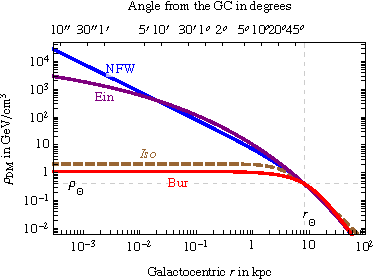
\includegraphics[width=\textwidth]{figs/DMprofiles}
\end{minipage}
\quad
\begin{minipage}{0.4\textwidth}
\centering
\footnotesize{  
\begin{tabular}{l|rc}
DM halo &   $r_{s}$ in kpc& $\rho_{s}$ in GeV/cm$^{3}$\\
  \hline \\[-1mm]
  NFW  & 14.46 & 0.566 \\ \\
  Einasto  & 13.63 & 0.154 \\ \\
  Burkert  & 10.62 & 1.143 \\ \\
 {\it Isothermal} & {\it 4.00} & {\it 2.112} \\
 \end{tabular}} 
\label{tab:profiles}
\end{minipage}
\caption[DM galactic density profiles $\rho(r)$]{\em \label{fig:DMprofiles} {\bfseries DM profiles} (figure left) and (table right) the corresponding parameters in the parametrizations of the profiles in  Table \ref{eq:profiles}. The procedure to determine the parameters of the Isothermal profile is different from the other ones, see the text for details.  
In the table we provide $r_s$ ($\rho_s$) to 2 (3) significant digits, a precision sufficient for most computations. Still more precise inputs are needed in specific cases, such as to precisely reproduce the $J$ factors (discussed in section~\ref{sec:IDgamma}) for small angular regions around the Galactic Center.}
\end{figure}

\setstretch{1}
\subsection[Milky Way parameters]{Determination of the Milky Way parameters}\label{sec:MilkyWay}
\index{DM abundance!local}


\renewcommand{\arraystretch}{0.7}
\begin{table}[!t]
\begin{center}
\small{
\begin{tabular}{l|c|c|l}
\bf Authors & \bf Date & \bfseries{$\rho_\odot$  in GeV/cm$^3$} & \bf  Notes \\[1mm]
\hline
& &  & \\[-3mm] \rowcolor[rgb]{0.95,0.97,0.97}
Turner 				& 1986	& 0.28 & {`uncertainty of about a factor of 2'}\\[1mm] \rowcolor[rgb]{0.95,0.97,0.97}
Flores 				& 1988	& $0.3 \leftrightarrow 0.43$ & \\[1mm] \rowcolor[rgb]{0.95,0.97,0.97}
Kuijken \& Gilmore		& 1991 	& $0.42\ (\pm 20\%)$ & \\[1mm]
\hdashline \rowcolor[rgb]{0.97,0.97,0.93}
& & &  \\[-2mm] \rowcolor[rgb]{0.97,0.97,0.93}
Widrow et al. 			& 2008 	& $0.304 \pm 0.053$ & \\[1mm] \rowcolor[rgb]{0.97,0.97,0.93}
Catena \& Ullio 			& 2009  	& $0.385 \pm 0.027$ & {Einasto} \\ \rowcolor[rgb]{0.97,0.97,0.93}
					& 		& $0.389 \pm 0.025$ & {NFW} \\[1mm] \rowcolor[rgb]{0.97,0.97,0.93}
Weber \& de Boer 		& 2009 	& $0.2 \leftrightarrow 0.4$ & \\[1mm] \rowcolor[rgb]{0.97,0.97,0.93}
Salucci et al. 			& 2010 	& $0.43\pm0.11\pm0.10$ & \\[1mm] \rowcolor[rgb]{0.97,0.97,0.93}
McMillan 				& 2011 	& $0.40 \pm 0.04$ & \\[1mm]	 \rowcolor[rgb]{0.97,0.97,0.93}
Garbari et al. 			& 2011 	& $0.11^{+0.34}_{-0.27}$ & {isothermal stellar tracers} \\[0.6mm] \rowcolor[rgb]{0.97,0.97,0.93}
					& 		& $1.25^{+0.30}_{-0.34}$ & {non-isothermal stellar tracers} \\[1mm]\rowcolor[rgb]{0.97,0.97,0.93}
Iocco, Pato \& Bertone	& 2011	& $0.2 \to 0.56$	& 	\\[1mm]	\rowcolor[rgb]{0.97,0.97,0.93}
Bovy \& Tremaine 		& 2012 	& $0.3\pm0.1$ & \\[1mm]\rowcolor[rgb]{0.97,0.97,0.93}
Zhang et al. 			& 2012 	& $0.28 \pm 0.08$ & \\[1mm]\rowcolor[rgb]{0.97,0.97,0.93}
Piffl et al. 				& 2014 	& $0.59\ (\pm 15\%)$ & \\[1mm]\rowcolor[rgb]{0.97,0.97,0.93}
Pato, Iocco \& Bertone 	& 2015 	& $0.420 \pm 0.025$ &  \\[1mm]\rowcolor[rgb]{0.97,0.97,0.93}
McKee et al.			& 2015 	& $0.49 \pm 0.13$ &  \\[1mm]\rowcolor[rgb]{0.97,0.97,0.93}
McMillan 				& 2016 	& $0.40 \pm 0.04$ &  \\[1mm]\rowcolor[rgb]{0.97,0.97,0.93}
Sivertsson et al.		& 2017 	& $0.46^{+0.07}_{-0.09}$ &  \\[1mm]
\hdashline \rowcolor[rgb]{0.99,0.97,0.97}
& & &  \\[-2mm] \rowcolor[rgb]{0.99,0.97,0.97}
Buch et al. 			& 2018 	& $0.608 \pm 0.380$ &  {result depends on chosen tracers}  \\[1mm] \rowcolor[rgb]{0.99,0.97,0.97}
Eilers et al.			& 2018	& $0.30 \pm 0.03$ & \\[1mm]\rowcolor[rgb]{0.99,0.97,0.97}
Evans et al.			& 2018	& $0.55 \pm 0.17$ & \\[1mm]\rowcolor[rgb]{0.99,0.97,0.97}
Karukes et al. 			& 2019 	& $0.43 \pm 0.02 \pm 0.01 $ &  {stat and sys errors}  \\[1mm]\rowcolor[rgb]{0.99,0.97,0.97}
Cautun et al.			& 2020	& $0.33 \pm 0.02$ & \\[1mm]\rowcolor[rgb]{0.99,0.97,0.97}
Sofue				& 2020	& $0.359 \pm 0.017$ & {own determination} \\\rowcolor[rgb]{0.99,0.97,0.97}
					& 		& $0.39 \pm 0.09$ & {average of recent results} \\[1mm]\rowcolor[rgb]{0.99,0.97,0.97}
Salomon et al.			& 2020	& $0.42 \leftrightarrow 0.53 $ & \\[1mm]		\rowcolor[rgb]{0.99,0.97,0.97}				
Hattori et al.			& 2020	& $0.342 \pm 0.007$ & \\[1mm]		\rowcolor[rgb]{0.99,0.97,0.97}			
Benito, Iocco \& Cuoco 	& 2021 	& $0.4 \leftrightarrow 0.7$ & {inferred 2$\sigma$ range} \\[1mm]	\rowcolor[rgb]{0.99,0.97,0.97}
Lim, Putney, Buckley, Shih 	& 2023 	& $0.446 \pm 0.054$ & \\[1mm]	\rowcolor[rgb]{0.99,0.97,0.97}
Staudt et al. 			& 2024	& $0.42 \pm 0.06$  & from simulations
\end{tabular}}
\end{center}
\vspace{-5mm}
\caption[DM density at the location of the Sun]{\em\label{tab:rhodot} {\bfseries DM density at the location of the Sun}. The top set consists of `historical' studies. The bottom set contains a selection of works published after the release of {\sc Gaia} data (although not necessarily using them). The middle set lists selected results of the latest $\sim 15$ years. Note that the position of the Sun may not be exactly the same for all authors, that the methods are different, that the key assumptions might differ, and that relative renormalizations might be necessary. References are in~\cite{rhoSun}. }
\end{table}
\renewcommand{\arraystretch}{1}


Next, one has to determine the parameters $r_s$ (typical scale radius) and $\rho_s$ (typical scale density) that enter in 
the tentative DM distributions $\rho(r)$. This can be done in different ways, e.g., by extracting their values from numerical simulations of Milky Way-like halos, or determining them in some way from observations of the Milky Way or similar outer galaxies.  
One approach 
is to impose that the DM profiles for the Milky Way satisfy the following set of constraints:
\begin{itemize}
\item[A)] The {\bf density of Dark Matter at the location}\footnote{The distance of the Sun from the Galactic Center~\cite{rSun} is also somewhat uncertain. In recent years the central value has fluctuated around 8.3 kpc, with an error of about $\pm 0.3$ kpc. One of the most recent and most precise determinations, due to the {\sc Gravity} collaboration~\cite{rSun}, yields $r_\odot= 8.277 \pm 0.031$  kpc (statistical and systematic errors summed in quadrature).} {\bf of the Sun} $\rho_\odot$.
This quantity was studied by many groups using a number of different techniques~\cite{rhoSun}, notably the {\it global method} of fitting the entire rotation curve of the Galaxy, as discussed above, or the {\it local methods}, which rely on studying local stellar kinematics (especially the stellar motions in the vertical direction) to determine the local gravitational pull and therefore the local DM density. 
The global method can provide a precise determination of $\rho_\odot$, but is sensitive to the uncertain modeling of the baryonic components of the Galaxy.
The local methods are less precise and suffer, on one hand, from the systematics due to peculiar local conditions (such as the asymmetries in the north and south galactic hemispheres) and, on the other hand, from the simplifications in the analysis (e.g., whether or not the so-called `tilt term', which correlates radial and vertical stellar motions, is included).

The recent determinations of $\rho_\odot$ point towards 
\beq
\label{eq:rhosun:value}
\bbox{\rho_\odot=\rho(r_\odot) = 0.40 \, \GeV/{\rm cm}^{3} \approx 0.0106 \, M_\odot/{\rm pc}^{3}}.
\eeq
The typical associated error  is $\pm 0.10$ GeV/cm$^{3}$, 
but a possible spread up to $0.2 \leftrightarrows 0.8$ GeV/cm$^{3}$ (sometimes referred to as `a factor of 2') is often adopted. As is evident from the selected results listed in table~\ref{tab:rhodot}, different determinations of $\rho_\odot$ are still in poor agreement. Historically, the conventional value used in the literature since the 1990s used to be $\rho_\odot = 0.3 \, \GeV/{\rm cm}^{3}$. This value increased following several studies, performed mostly between 2009 and 2011, which found somewhat higher central values. 
Other studies, on the other hand,  found smaller central values.\footnote{In 2012 the result from \arxivref{1204.3924}{Moni Bidin et al.}~\cite{rhoSun} made the news, since they found $\rho_\odot = 0.000\pm0.004 \ {\rm GeV}/{\rm cm}^3$, later ascribed to poor modeling.} 
Additionally, the associated error remained a topic of intense debate.
Data from the {\sc Gaia} mission stimulated new activities aimed at determining $\rho_\odot$, but the situation is not yet  settled, and a more precise determination of $\rho_\odot$ seems difficult to achieve.
\end{itemize}
For comparison, the total matter density (including normal matter) averaged over a neighborhood of a few hundred parsecs around the location of the Sun is estimated to be an order of magnitude larger than the DM density~\eqref{eq:rhosun:value}~\cite{1711.07504}, 
\beq  4.5 \, {\rm GeV}/{\rm cm}^{3} \approx 0.120 \, M_\odot/{\rm pc}^{3}.\eeq
Eq.\eq{rhosun:value} means that the mass of the Dark Matter included within the orbit of Neptune ($\sim 30$ AU) is of the order of $10^{-13} M_\odot$ or, equivalently, that the mass of the Sun corresponds to the mass of all the Dark Matter contained in a sphere of radius $2.8\,{\rm pc} \approx 9.2 \,{\rm ly}$, comparable to the distance to the nearest star, about $4$ ly. 
This illustrates how DM is largely subdominant locally. One may wonder whether its presence in the solar system could nevertheless be detected via its influence on the orbits of planets and the closely monitored asteroids (for one, the accumulated DM would slightly increase the effective mass of the Sun as seen by the outer bodies). However, direct astronomical observations, while accurate, are still not particularly constraining. The resulting bound on DM density in the solar system is $\rho \circa{<} 5000\GeV/\cm^3$, which is about 15000 times larger than the expected $\rho_\odot$~\cite{DMsolarsystem}. In other words, DM has no significant effect on the orbits of the planets in the solar system. 

A related issue is whether the average value for $\rho_\odot$ in eq.\eq{rhosun:value} can be modified significantly by the presence of astrophysical bodies in the solar system, e.g., whether it could get increased by the gravitational attraction of the Sun or decreased by slingshot effects acting on DM particles passing the planets (notably Jupiter, but also Venus and the Earth itself, in the same way as what happens for conventional asteroids). Any appreciable modification of local DM density and speed distributions would be particularly important for the interpretations of DM direct detection results (see chapter \ref{chapter:direct}), and for predicting the neutrino flux from DM particles captured in the Sun or the Earth (see section \ref{sec:DMnu}). A series of detailed studies identified a number of subtle effects that, for the most part, cancel each other out, leading to a practically negligible net effect, at least for DM particles that interact only weakly with the astrophysical bodies~\cite{DMdensitysolarsystem}.

\smallskip

Note also that the energy density in DM is  $\rho_\odot  \sim 20\,{\rm kW}/{\rm m}^2,$\footnote{Using $c=1$ units. One can think of it as the maximal energy flux seen by an observer moving at the speed of light, if all DM rest mass were to be absorbed. 
If the observer is effectively at rest (e.g.~on Earth), and is hit by the DM flux with speed $v \sim 10^{-3} c$, then the hypothetically available energy density is $10^{-3}$ times smaller.
In any case, since DM interacts only feebly with matter (if at all), the probability of DM actually being absorbed is minuscule, making it exceedingly hard to tap into this source of energy.} about 14 times higher than the power density of the Sun's radiation on the surface of the Earth (good to keep in mind, just in case this energy someday turns out to be in a usable form, converting our universe into one giant battery pack).






\begin{itemize}
\item[B)] The {\bf total DM mass contained in the Milky Way}. This quantity was also studied by many groups, using different techniques~\cite{MWmass}. The methods include the study of the kinematics of bright satellites (such as the dwarf galaxies or the Magellanic clouds), the kinematics of stellar streams, the escape velocity of nearby rogue stars and the use of various tracers.
For $M^{\rm DM}_{200}$, the mass of Dark Matter contained inside a virial radius $r_{200}$, defined in section~\ref{sec:rho_from_analytic} (below eq.~\eqref{eq:rhovir}), we will use 
 the `standard' value
\beq
\label{eq:M200:value}
\bbox{M^{\rm DM}_{200}\equiv (1.0 \pm 0.25) \times 10^{12} \, M_\odot}.
\eeq
However, it is worth noting that the advent of the {\sc Gaia} mission and its precise astrometric data resulted in a lot of activity recently, with a number of studies in 
2023 arriving at a factor of a few lower value for $M^{\rm DM}_{200}$~\cite{rotation_curves}. 
For the Milky Way,
$r_{200}\sim 200\,\text{to}\,300$ kpc, hence one can think of $M^{\rm DM}_{200}$ as the total DM mass contained in a large sphere of radius 200 kpc centered around the center of the Galaxy.
\end{itemize}
For comparison, the stellar mass inferred with similar techniques is $\approx 8 \times 10^{10}\, M_\odot$. The distance from the Earth to the Large Magellanic Cloud, is about 48.5 kpc.

\medskip

Imposing the constraints (\ref{eq:rhosun:value}) and (\ref{eq:M200:value}) fixes the $r_s$ and $\rho_s$ parameters\footnote{We should stress that the different parameters discussed in these sections ($\rho_\odot, r_\odot$, $M^{\rm DM}_{200}$ and, later on, the rotational velocity of the Sun) are interconnected and correlated. As discussed above, they are typically determined within a global galactic model, which consists of the baryonic components but often also requires to specify a DM density distribution and a DM velocity distribution. Hence, strictly speaking, using the values $\rho_\odot, r_\odot$ and $M^{\rm DM}_{200}$ to constrain the DM distributions is inconsistent. However, the impact of the choice of the DM distributions on the global model is limited, thus the procedure can be considered as valid for all current practical purposes.} 
for the NFW, Einasto and Burkert profiles in table~\ref{eq:profiles}. For the Isothermal profile, however, no solution can be found that would simultaneously satisfy both constraints: the $r^{-2}$ behavior of DM density at large $r$ is too slow and always results in $M^{\rm DM}_{200}$  larger than the value in eq.~(\ref{eq:M200:value}). For this profile we therefore disregard the constraint in eq.~(\ref{eq:M200:value}); instead we set $r_s = 4$ kpc, as was done in the original literature, and then determine the value of $\rho_s$ for which the constraint on the local density in eq.~(\ref{eq:rhosun:value}) is satisfied.
The results of this procedure are presented in fig.~\ref{fig:DMprofiles}, where we also plot the resulting profiles. 
The values of the parameters determined with this procedure, and presented here, in general 
do not differ much, at most by 20\%, from the parameter values often used 
in the literature.



\subsection{Dwarf galaxies}\index{Dwarf galaxies}\index{DM abundance!dwarf galaxies}
\label{sec:dwarfs}

\begin{table}[p]
\vspace{-0.6cm} 
\begin{center}
\setlength\tabcolsep{4pt} \renewcommand{\arraystretch}{1.25}
\scriptsize{
\hspace*{-1.cm} 
\begin{tabular}{cl|c|c|c|c||rl|rl} 
& {\bf Name} & {\bf Discovery} & {\bf Position} & {\bf Distance}  & $r_{\rm HL}$ & \multicolumn{2}{c|}{${\rm log}_{10}\,{\mathcal J}_{\rm dSph} ({\rm disk}_{0.5^\circ})$} & \multicolumn{2}{c}{${\rm log}_{10}\,{\mathcal D}_{\rm dSph} ({\rm disk}_{0.5^\circ})$} \\[0.1mm]
& 		 & 	 &  ($b, \ell$) & in kpc & in pc & \multicolumn{2}{c|}{in ${\rm GeV}^2 \, {\rm cm}^{-5}$} & \multicolumn{2}{c}{in ${\rm GeV} \, {\rm cm}^{-2}$} \\[0.5mm]
\hline
 & & &  & & & &	\\[-4mm]
\multirow{8}{*}{\rotatebox[origin=c]{270}{{\it classical}}} 
& Sculptor		& 1938 & $(-83.2^\circ, 287.5^\circ$)		& 86 $\pm$6 	& 283 $\pm$45	& \quad $18.58$&$^{+0.05}_{-0.05}$ 	& \quad $18.20$&$^{+0.09}_{-0.08}$ \\
& Fornax  		& 1938 & $(-65.7^\circ, 237.1^\circ$) 	& 147 $\pm$12 & 710 $\pm$77	& $18.09$&$^{+0.10}_{-0.10}$	& $17.97$&$^{+0.05}_{-0.05}$ \\
& Leo I 		& 1950 & $(+49.1^\circ, 226.0^\circ$)	& 254 $\pm$15 & 251 $\pm$27	& $17.61$&$^{+0.13}_{-0.11}$	& $18.01$&$^{+0.20}_{-0.28}$ \\
& Leo II 		& 1950 & $(+67.2^\circ, 220.2^\circ$) 	& 233 $\pm$14 & 176 $\pm$42 & $17.66$&$^{+0.16}_{-0.15}$	& $17.64$&$^{+0.50}_{-0.33}$ \\
& Ursa Minor 	& 1955 & $(+44.8^\circ, 105.0^\circ$) 	& 76 $\pm$3 	& 181 $\pm$27 & $18.76$&$^{+0.12}_{-0.11}$	& $18.20$&$^{+0.14}_{-0.08}$ \\
& Draco 		& 1955 & $(+34.7^\circ, 86.4^\circ$)  	& 76 $\pm$6	& 221 $\pm$19	& $18.82$&$^{+0.12}_{-0.12}$	& $18.54$&$^{+0.11}_{-0.14}$ \\
& Carina 		& 1977 & $(-22.2^\circ, 260.1^\circ$) 	& 105 $\pm$6 	& 250 $\pm$39 & $17.83$&$^{+0.09}_{-0.09}$	& $17.88$&$^{+0.18}_{-0.15}$ \\
& Sextans 	& 1990 & $(+42.3^\circ, 243.5^\circ$) 	& 86 $\pm$4 	& 695 $\pm$44	& $17.75$&$^{+0.12}_{-0.11}$	& $17.90$&$^{+0.11}_{-0.09}$ \\[1mm]
\hdashline
& & & & & & & & \\[-4mm]
& Sagittarius 	& 1994 & $(-14.2^\circ, 5.6^\circ$) 		& 26 $\pm$2 	& 2587 $\pm$219 & $19.77$&$^{+0.08}_{-0.07} \ \ \ast$	& \multicolumn{2}{c}{$-$}	\\[1mm]
\hdashline 
& & & & & & & & \\[-4mm]
\multirow{20}{*}{\rotatebox[origin=c]{270}{{\it confirmed ultrafaint}}} 
& Willman 1 		& 2005 {\scriptsize (SDSS)} & $(+56.8^\circ, 158.6^\circ$) 	& 38 $\pm$7 	& 25 $\pm$6			& $19.36$&$^{+0.52}_{-0.46}$ 		& $18.52$&$^{+0.47}_{-0.68}$ \\
& Ursa Major I 		& 2005 {\scriptsize (SDSS)} & $(+54.4^\circ, 159.4^\circ$) 	& 97 $\pm$4 	& 319 $\pm$50			& $18.33$&$^{+0.28}_{-0.28} \ \ \ast$ 	& $18.10$&$^{+0.28}_{-0.29} \ \ \ast$ \\
& Ursa Major II 		& 2006 {\scriptsize (SDSS)} & $(-37.4^\circ, 152.5^\circ$)		& 32 $\pm$4  	& 149 $\pm$21 		& $19.44$&$^{+0.41}_{-0.39}$ 		& $18.64$&$^{+0.28}_{-0.31}$ \\
& Bo\"otes I 		& 2006 {\scriptsize (SDSS)} & $(+69.6^\circ, 358.1^\circ$) 	& 66 $\pm$2 	& 242 $\pm$21 		& $18.19$&$^{+0.30}_{-0.28}$		& $18.11$&$^{+0.25}_{-0.30}$ \\
& Canes Venatici I 	& 2006 {\scriptsize (SDSS)} & $(+79.8^\circ, 74.3^\circ$) 		& 218 $\pm$10 & 564 $\pm$36 		& $17.43$&$^{+0.16}_{-0.15}$		& $17.79$&$^{+0.26}_{-0.27}$ \\
& Canes Venatici II 	& 2006 {\scriptsize (SDSS)} & $(+82.7^\circ, 113.6^\circ$)		& 160 $\pm$4	& 74 $\pm$14 			& $17.82$&$^{+0.48}_{-0.47}$		& $18.01$&$^{+0.36}_{-0.51} \ \ \ast$ \\
& Coma Berenices 	& 2007 {\scriptsize (SDSS)} & $(+83.6^\circ, 241.9^\circ$) 	& 44 $\pm$4 	& 77 $\pm$10 			& $19.01$&$^{+0.36}_{-0.36}$		& $18.45$&$^{+0.29}_{-0.44}$ \\
& Hercules 		& 2007 {\scriptsize (SDSS)} & $(+36.9^\circ, 28.7^\circ$) 		& 132 $\pm$12	& $330 \ ^{+75}_{-52}$ 	& $17.29$&$^{+0.51}_{-0.52} \ \ \ast$	& $17.52$&$^{+0.50}_{-0.51} \ \ \ast$ \\
& Leo IV 			& 2007 {\scriptsize (SDSS)} & $(+57.4^\circ, 264.4^\circ$) 	& 154 $\pm$6	& 206 $\pm$37 		& $16.40$&$^{+1.01}_{-1.15} \ \ \ast$ 	& $16.74$&$^{+0.55}_{-0.56} \ \ \ast$ \\
& Segue 1			& 2007 {\scriptsize (SDSS)} & $(+50.4^\circ, 220.5^\circ$)  	& 23 $\pm$2	& $29 \ ^{+8}_{-5}$ 		& $19.00$&$^{+0.48}_{-0.68}\ \  \ast$	& $18.08$&$^{+0.53}_{-0.49} \ \ \ast$ \\
& Leo T 			& 2007 {\scriptsize (SDSS)} & $(+43.7^\circ, 214.9^\circ$) 	& 417 $\pm$19 & 120 $\pm$9			& $17.49$&$^{+0.49}_{-0.45}$		& $17.67$&$^{+0.53}_{-0.60}$ \\
& Leo V 			& 2008 {\scriptsize (SDSS)} & $(+58.5^\circ, 261.9^\circ$) 	& 178 $\pm$10	& 135 $\pm$32 		& $17.65$&$^{+0.91}_{-1.03} \ \ \ast$	& $17.13$&$^{+0.65}_{-0.72}$ \\
& Segue 2 		& 2009 {\scriptsize (SDSS)} & $(-38.1^\circ, 149.4^\circ$) 		& 35 $\pm$2 	& 35 $\pm$3			& $16.21$&$^{+1.08}_{-0.98} \ \ \ast$	& $15.89$&$^{+0.56}_{-0.37} \ \ \ast$ \\
& Sagittarius II 		& 2015 {\scriptsize (Pan-STARRS)} & $(-22.9^\circ, 18.9^\circ$) & 67 $\pm$5 	& $38 \ ^{+8}_{-7}$		& $17.35$&$^{+1.36}_{-0.91} \ \ \ast$ 	& \multicolumn{2}{c}{$-$} \\ 
& Reticulum II 		& 2015 {\scriptsize (DES)} & $(-49.7^\circ, 266.3^\circ$) 		& 31.4 $\pm1.4$ 	& 58 $\pm4$		& $18.94$&$^{+0.38}_{-0.38} \ \ \ast$	& $18.30$&$^{+0.33}_{-0.50} \ \ \ast$  \\ 
& Eridanus II 		& 2015 {\scriptsize (DES)} & $(-51.6^\circ, 249.8^\circ$) 		&  380 			&  158			& $17.28$&$^{+0.34}_{-0.31}$ 		& $17.60$&$^{+0.42}_{-0.54}$ \\ 
& Tucana II 		& 2015 {\scriptsize (DES)} & $(-52.3^\circ, 328.1^\circ$) 		& 57 $\pm5$ 		& $165 \ ^{+28}_{-19}$	& $18.93$&$^{+0.56}_{-0.50}$ 	& $18.46$&$^{+0.35}_{-0.36}$  \\
& Horologium I 		& 2015 {\scriptsize (DES)} & $(-54.7^\circ, 271.4^\circ$) 		&  79				&  31				& $19.17$&$^{+0.80}_{-0.70}$ 		& $18.14$&$^{+0.65}_{-0.63}$ \\
& Phoenix II 		& 2015 {\scriptsize (DES)} & $(-59.7^\circ, 323.7^\circ$) 		& 84.1 $\pm$ 8 	& 37 $\pm$ 8		& $18.20$ &			 		& \multicolumn{2}{c}{$-$} \\ 
& Tucana IV 		& 2015 {\scriptsize (DES)} & $(-55.3^\circ, 313.3^\circ$) 		& 48 $\pm4$ 		& 127 $\pm24$		& $(18.7)$  &					& \multicolumn{2}{c}{$-$} \\
& Aquarius II 		& 2016 {\scriptsize (SDSS)} & $(-53.0^\circ, 55.1^\circ$) 		&  108		 	&  125			& $18.39$&$^{+0.65}_{-0.58}$ 		& $18.07$&$^{+0.47}_{-0.50}$ \\
& Crater II 		& 2016 {\scriptsize (ATLAS)} 	& $(+42.2^\circ, 282.9^\circ$) 	&  117 $\pm$ 1	 	&  1066 $\pm$ 84	& \multicolumn{2}{c|}{$-$}	 		& \multicolumn{2}{c}{$-$} \\
& Carina II		& 2018 {\scriptsize (MagLiteS)} & $(-17.1^\circ, 269.9^\circ$) 	&  36 			&  77				& $18.37$&$^{+0.54}_{-0.52}$ 		& $17.95$&$^{+0.38}_{-0.40}$ \\
& Carina III		& 2018 {\scriptsize (MagLiteS)} & $(-16.8^\circ, 270.0^\circ$) 	&  28				& 20				& $20.2$&$^{+1.0}_{-0.9}$		& $18.8$&$^{+0.6}_{-0.7}$ \\
& Antlia II 			& 2019 {\scriptsize (Gaia)} 	& $(+11.2^\circ, 264.9^\circ$) 	&  132 			& 2301			& \multicolumn{2}{c|}{$-$} 			& \multicolumn{2}{c}{$-$} \\
& Pegasus IV 		& 2022 {\scriptsize (DELVE)} 	& $(-21.4^\circ, 80.8^\circ$) 	&  $90\ ^{+4}_{-6}$		& $41\ ^{+8}_{-8}$		& \multicolumn{2}{c|}{$-$} 			& \multicolumn{2}{c}{$-$} \\
& Virgo II 			& 2022 {\scriptsize (DELVE)} 	& $(+52.8^\circ, 4.1^\circ$) 	&  $72\ ^{+8}_{-7}$		& 16	$\pm3$		& \multicolumn{2}{c|}{$-$} 			& \multicolumn{2}{c}{$-$} \\
& Bo\"otes V 		& 2022 {\scriptsize (DELVE/UNIONS)} & $(+70.9^\circ, 55.7^\circ$) 	&  102 $\pm 21$		& 20	$\pm7$		& \multicolumn{2}{c|}{$-$} 			& \multicolumn{2}{c}{$-$} \\
& Leo Minor I 		& 2022 {\scriptsize (DELVE)} 	& $(+64.7^\circ, 202.2^\circ$) 	&  $82\ ^{+4}_{-7}$		& 26	$\pm9$		& \multicolumn{2}{c|}{$-$} 			& \multicolumn{2}{c}{$-$} \\
\hdashline
& & & & & & & &  \\[-4mm]
\multirow{14}{*}{\rotatebox[origin=c]{270}{{\it candidates}}}
& Triangulum II 		& 2015 {\scriptsize (Pan-STARRS)} 	& $(-23.4^\circ, 141.4^\circ$) 	& 30 $\pm$2  	& 28 $\pm$8		& $19.35$&$^{+0.37}_{-0.37} \ \ \ast$	& $18.42$&$^{+0.86}_{-0.79} \ \ \ast$ \\
& Draco II 		& 2015 {\scriptsize (Pan-STARRS)} 	& $(+42.9^\circ, 98.3^\circ$) 	& 20 $\pm$3 	& $19 \ ^{+8}_{-6}$ 	& $18.93$&$^{+1.39}_{-1.70} \ \ \ast$	& $18.02$&$^{+0.84}_{-0.87} \ \ \ast$ \\
& Pictor I 			& 2015 {\scriptsize (DES)} 		& $(-40.6^\circ, 257.3^\circ$) 	& 114 		& 18				& \multicolumn{2}{c|}{$-$}			& \multicolumn{2}{c}{$-$}  \\
& Grus I	 		& 2015 {\scriptsize (DES)} 		& $(-58.2^\circ, 338.7^\circ$) 	& 120	 	&  21				& $16.88$&$^{+1.51}_{-1.66}$		& $17.00$&$^{+0.87}_{-0.86}$ \\
& Grus II	 		& 2015 {\scriptsize (DES)} 		& $(-51.9^\circ, 351.1^\circ$) 	& 53 $\pm5$ 	& 93 $\pm14$		& $(18.7)$	 &					& \multicolumn{2}{c}{$-$}  \\
& Tucana III 		& 2015 {\scriptsize (DES)} 		& $(-56.2^\circ, 315.4^\circ$) 	& 25 $\pm2$ 	& 44 $\pm6$		& $(19.4)$	 &					& \multicolumn{2}{c}{$-$}  \\
& Columba I 		& 2015 {\scriptsize (DES)} 		& $(-28.9^\circ, 231.6^\circ$) 	& 183 		& 98				& \multicolumn{2}{c|}{$-$}			& \multicolumn{2}{c}{$-$}  \\
& Reticulum III 		& 2015 {\scriptsize (DES)} 		& $(-45.6^\circ, 273.9^\circ$) 	&  92	 		& 64				& \multicolumn{2}{c|}{$-$}			& \multicolumn{2}{c}{$-$}  \\
& Tucana V 		& 2015 {\scriptsize (DES)} 		& $(-51.9^\circ, 316.3^\circ$) 	&  55			& 16				& \multicolumn{2}{c|}{$-$}			& \multicolumn{2}{c}{$-$}  \\
& Indus II 			& 2015 {\scriptsize (DES)} 		& $(-37.4^\circ, 354.0^\circ$) 	&  214	 	& 180			& \multicolumn{2}{c|}{$-$}			& \multicolumn{2}{c}{$-$}  \\
& Cetus II 			& 2015 {\scriptsize (DES)} 		& $(-78.5^\circ, 156.5^\circ$) 	&  30		 	& 17				& \multicolumn{2}{c|}{$-$}			& \multicolumn{2}{c}{$-$}  \\
& Virgo I			& 2016 {\scriptsize (HSC)} 		& $(+59.6^\circ, 276.9^\circ$) 	&  $91\ ^{+9}_{-4}$		& $47\ ^{+19}_{-13}$		& \multicolumn{2}{c|}{$-$}			& \multicolumn{2}{c}{$-$}  \\
& Cetus III			& 2018 {\scriptsize (HSC)} 		& $(-61.1^\circ, 163.8^\circ$) 	&  $251\ ^{+24}_{-11}$	& $90\ ^{+42}_{-17}$		& \multicolumn{2}{c|}{$-$}			& \multicolumn{2}{c}{$-$}  \\
& Bo\"otes IV		& 2018 {\scriptsize (HSC)} 		& $(+53.3^\circ, 70.7^\circ$) 	&  $209\ ^{+20}_{-18}$ 	&  $462\ ^{+98}_{-84}$	& \multicolumn{2}{c|}{$-$}			& \multicolumn{2}{c}{$-$} \\  
& Centaurus I		& 2019 {\scriptsize (DELVE)} 		& $(+21.9^\circ, 300.3^\circ$) 	&  $116.3\ ^{+1.6}_{-0.6}$ 	&  $79\ ^{+14}_{-10}$	& \multicolumn{2}{c|}{$-$}			& \multicolumn{2}{c}{$-$} \\
& Eridanus IV		& 2021 {\scriptsize (DELVE)} 		& $(-27.8^\circ, 209.5^\circ$) 	&  $76.6\ ^{+4.0}_{-6.1}$ 	&  $75\ ^{+16}_{-13}$	& \multicolumn{2}{c|}{$-$}			& \multicolumn{2}{c}{$-$} \\
& Ursa Major III		& 2023 {\scriptsize (UNIONS)} 		& $(+73.7^\circ, 194.6^\circ$) 	&  10 $\pm 1$ 			&  $3\ \pm 1$			& $20.87$&$^{+0.60}_{-0.58} \ \ \ast$& \multicolumn{2}{c}{$-$}
 \end{tabular}}
\end{center}
\vspace{-7mm}
\caption[Dwarf galaxies]{\em \footnotesize \label{tab:dwarfs} Most of the discovered {\bfseries dwarf spheroidal satellite galaxies} of the Milky Way. Data are from many different sources~\cite{dwarfgalaxies,Jdwarfs}, and not necessarily with homogenous methods. The ${\mathcal J}_{\rm dSph}$ and ${\mathcal D}_{\rm dSph}$ factors are defined in eq.\eq{JdSph} (${\mathcal D}$ is proportional to the dwarf's mass due to DM) and are computed for a $0.5^\circ$ disk.  
 The cases with particularly large variations in the literature ($\mathcal{O}(10)$ in the central value) are labeled with $\ast$. The values in parenthesis are estimates.}
\end{table}


The Milky Way is surrounded by a number of {\it satellite galaxies}~\cite{dwarfgalaxies}, i.e.,~astrophysical systems that are tied to the main MW halo by gravitational attraction. Apart from the Large and Small Magellanic Clouds, which are big enough to be seen with a naked eye, the large majority of the satellites consists of {\it dwarf galaxies}. 
Most of these are of the {\it dwarf spheroidal} (dSph) type and only a few are dwarf irregulars (dIrr). 
Historically, Sculptor was the first one to be discovered (in 1938) and it is often considered as the prototypical dSph. Seven more dwarf galaxies (Fornax, Leo I, Leo II, Ursa Minor, Draco, Carina and Sextans) were discovered up to the 1990s. Collectively, these 8 dwarf galaxies are referred to as {\it classical}. With the advent of the digital surveys such as {\sc Sdss}, the Subaru Hyper-Supreme Camera ({\sc Hsc}) (which covered the northern sky), {\sc Pan-Starrs}, {\sc Des} (which covered the southern sky) and {\sc Gaia} (operating from space), many more dwarfs have been discovered: these are referred to as {\it ultrafaint}. The current total stands just short of 50, including several whose nature and properties are not yet confirmed  (see table \ref{tab:dwarfs}).\footnote{
\arxivref{2302.02646}{Xu et al.~(2023)}~\cite{2302.02646} claim a discovery of the first DM-dominated dwarf galaxy external to the MW system. {\sc Fast} J0139+4328 is a (very large) dwarf galaxy located at about 29 Mpc which is found to have a DM-dominated ratio of total mass vs baryonic mass, $47\pm 27$.} The list is probably going to increase, as the surveys become more sensitive and cover larger portions of the sky, e.g.,~with the upcoming Rubin Observatory (formerly known as {\sc Lsst}). There is also the Sagittarius dSph, discovered in 1994, which is nearby and large, but stands apart, since it is believed to be tidally disrupted by the MW halo. 

The definition of the `dwarf' category is not clear cut, i.e.,~there are no universally accepted ranges of values for the mass, the size, and the luminosity of a small galaxy that would define it as being of the dwarf type. 
In general, one can think of a dwarf galaxy as having a DM-dominated mass of around $10^6 \, M_\odot$ (see fig.\fig{catalogue}),
where the actual dwarf galaxies can differ by a couple of orders of magnitude from this value: for instance, Fornax is estimated at $56 \cdot 10^6 \, M_\odot$ while Segue 2 at $0.23 \cdot 10^6 \, M_\odot$~\cite{dwarfgalaxies}. 
The half-light radius $r_{\rm HL}$, defined as the radius of a circle\footnote{For objects with a very elliptical shape, a `half-light ellipse' with different major and minor axes is sometimes defined. Spherical symmetry is however usually assumed for simplicity.} that contains half of the light emission from the galaxy, can be from a few tens of parsecs to several hundred parsecs. According to simulations, the virial radius $r_{200}$ of the DM halo of the dwarf galaxy tends to be one order of magnitude bigger than $r_{\rm HL}$~\cite{1801.06222}. The number of stars identified as belonging to the dwarf galaxy can be as low as a dozen or as many as several thousand. 



\medskip


Dwarf galaxies are  promising targets for DM searches, because they contain only a few stars and are believed to be dominated by Dark Matter. 
The likely reason is that dwarf galaxies constitute relatively shallow potential wells, compared to larger galaxies, facilitating the expulsion of baryonic gas by early supernov\ae{}, while 
 the subsequent star formation rate is low. 
 The estimated mass-to-light ratios $\Mcal _{\rm tot}/L$  can be of the order of several tens $M_\odot/L_\odot$ (e.g.,~Sculptor) to hundreds $M_\odot/L_\odot$ (e.g.,~Draco), and can even reach a few thousand $M_\odot/L_\odot$ (e.g.,~Segue 1).\footnote{Here, $L_\odot = 3.828 \cdot 10^{26}$ W is the nominal luminosity of the Sun, while $M_\odot = 1.9984 \cdot 10^{30}$ kg is the already encountered solar mass.} 
The large DM content of dwarfs is of course good news for the expected intensity of the DM signal. Moreover, the scarcity of stars and other active astrophysical objects implies that the signal is less contaminated by foreground emissions compared to other systems. However, this comes at the price of having only a small number of tracers with which one can reconstruct the DM content and the DM density profile. Also, these tracers are typically only stars: no hydrogen clouds, such as those that crucially helped in tracing the rotation curve of  spiral galaxies (see section~\ref{sec:evidencesmini}), are found in these systems.

\medskip


Because of stellar faintness and complex dynamics, the determinations of DM {\bf density functions} in dSphs are challenging and subject to intense debate. For example,  observationally there appears to be no consensus in the literature on whether the stellar kinematical data point to a cuspy or to a cored DM distribution.
A number of measurements, especially in the early 2000's, had suggested the preference for a core in the centers of dSphs. 
Subsequent observations showed, at least in the specific cases such as Sculptor and a few others, that a cusped NFW profile also fits the data well. 
The results of numerical simulations, on the other hand, seem to support the formation of cores for middle-sized dwarfs, while low mass dwarfs appear to develop cusps (consistent with the trend discussed in section~\ref{Nbody}). 
The core-vs-cusp  nature of dwarf galaxies might also depend on the history of star formation: dwarfs that stopped forming stars more than 6 Gyrs ago developed cusps by unimpeded contraction, while those that kept forming stars have had their DM content `heated' by stellar bursts and have thus developed cores.

A common practical approach in the literature involves using profiles like those discussed
in section~\ref{sec:DMdistribution}, with parameters determined in a number of different ways (see, e.g.,~\arxivref{1408.0002}{Geringer-Sameth (2015)} in~\cite{Jdwarfs}). From these one then predicts the corresponding DM signals (see section~\ref{sec:IDgammadSphs}).



\subsection{Galaxy clusters}\label{sec:clusters}
Galaxy clusters are the largest gravitationally bound systems in the Universe. 
They contain hundreds to thousands of galaxies, extend to several Mpc in size and have typical total masses up to $10^{14}- {\rm few}\ 10^{15}\, M_\odot$.
Galaxy clusters can be considered, in some respect, as a scaled-up version of galaxies, 
which provides a basic framework for understanding their principal characteristics (for detailed reviews see \cite{DMclusters}). 
However, significant differences also exist between galaxy clusters and galaxies.

\smallskip

Clusters contain baryonic and dark matter in proportions that are typically 1 to 10  (see section \ref{sec:evidencesmedi}). 
The formation of the DM halo of a cluster can be described, in first approximation, as the non-linear spherical collapse of an initial over-density, in a way which is entirely analogous to that described in section \ref{sec:rho_from_analytic} at the galactic scale. 
For more precise modeling, numerical simulations, which may include only dark matter or both dark matter and baryons, are employed.
These simulations show that the NFW and Einasto profiles introduced in section \ref{sec:DMdistribution} are good fits for the cluster DM distribution. 
This stresses that such profiles are roughly {\em universal} functions, i.e.~they apply to collapsed systems independently of their mass.
Like for galaxies, lensing observations seem however to show that the slope of the density profile in central regions of some clusters is shallower than predicted. 

\smallskip

Perhaps the most important qualitative difference between galaxies and galaxy clusters is that most baryons in clusters (as in the Universe) are in the form of diffuse gas, not stars. 
This implies a limited impact of baryonic physics in shaping the DM distribution: gas essentially only cools, and cooling does not have a major effect on the profiles (except very close to the inner regions of the cluster). 



\subsection{The halo mass function}\label{sec:haloMf}
\index{Halo mass function}\index{DM abundance!halo mass function}
In this section we compute the {\em halo mass function} $dn(t)/d\Mcal$: the average cosmological number density $n$ 
of gravitationally bound structures (galaxies, clusters of galaxies, dark matter halos, etc) with mass $\Mcal$, at a given time $t$.
Determining this quantity is interesting {\em per se}, since it is a fundamental prediction of the theory of structure formation. 
At the same time, the knowledge of $dn(t)/d\Mcal$ is also necessary for predicting the cosmological signals of DM annihilations.

The halo mass function $dn(t)/d\Mcal$ can be most accurately extracted from the numerical $N$-body  simulations (sections~\ref{Nbody}, \ref{sec:resNbody}). 
Historically, however, it has been determined using approximate analytic treatments~\cite{HaloMassFunction}, which, it turns out, reproduce surprisingly well the numerical results, despite some questionable assumptions and drastic simplifications. 
In the following, we review the analytical derivations, and mention how they have been improved in order to better agree with the simulations.

\smallskip

In section \ref{sec:linear:inhom} we reviewed the analytical theory of structure formation
in the limit $\delta(\vec x, t)\ll 1$, where $\delta$ is the density contrast. In this regime the Universe is still nearly homogeneous. Focusing on the period after matter/radiation equality (which is the one relevant for structure formation), all the modes of density perturbations that are well inside the horizon evolve in the same way,
so that $\delta(\vec x,t) = D(t/t') \delta(\vec x, t')$, where $\vec x$ is the comoving coordinate and $D$ is the so called  {\em growth factor}.
Below, we extrapolate these results to later times, when structures start to form. 
This may be questionable, since the gravitationally bound objects start to form when $\delta \sim 1$, i.e.,~in the mildly non-linear regime.
More precisely, both the analytical computations and the numerical simulations show that the structures form when $\delta>\delta_c$, where $\delta_c$ is the critical value of density contrast, equal to $\delta_c \approx 1.686$ for a spherically symmetric case. 
Extrapolating the small-$\delta$ regime up to $\delta\sim\delta_c$ is good enough for our purposes,
since $\delta_c$ is around unity.

We will assume that the density contrast $\delta$ follows a Gaussian distribution, see the discussion in the introduction to section \ref{sec:evidences}.
(In reality, $\delta\ge -1$, because density is positive, and thus the distribution needs to be truncated.) 
The variance of the density contrast distribution can be expressed as
\beq \sigma^2 = \frac{\int d^3x\, \delta^2(\vec x) }{\int d^3 x}=
\int \frac{d^3 k}{(2\pi)^3}  P(k)=\int\frac{dk}{k}\Delta^2(k),
\label{eq:sigmaforPS}
\eeq
where  $\Delta^2(k)=k^3 P(k)/2\pi^2$ is a dimension-less variance, while the power spectrum $P(k)$
was introduced in section~\ref{sec:linear:inhom}.
The variance $\sigma^2$ diverges, because the fluctuations are dominated by small scales, i.e.,\ large $k$.
This is cured by replacing $\delta(\vec x)$ with $\delta_R(\vec x)$, 
the density contrast smoothed over scales
of order $R$.
To perform the smoothing we introduce a `window function' $W_R(\vec x)$, which is sizable only within roughly a distance $R$ from the origin. This is then convoluted with $\delta$ to obtain:
\beq \delta_R(\vec x) = \int d^3x'\, \delta(\vec x') W_R(\vec x - \vec x'),
\qquad
\hbox{i.e.,}\qquad \delta_{Rk} = W(kR) \delta_k. 
\eeq
Here, $W(kR) = \int d^3 x \,W_R(\vec x)\exp(-i \vec k\cdot\vec x)$ is the Fourier transform of $W_R(\vec x)$.
The window function is normalised as $\int d^3x\, W_R(\vec x) = 1$.
Common choices are 
a sharp cut in $\vec k$ space ($W(kr) = 0$ outside a sphere $k<1/R$ and constant inside), or
a sharp cut in $\vec x$ space ($W_R(\vec x) = 0$ outside  $x>R$ and constant inside);
or a Gaussian function in both spaces ($W_R\propto e^{-r^2/2R^2}$, $W=e^{-k^2 R^2/2}$).

The variance of the smoothed inhomogeneity, computed analogously to eq.~(\ref{eq:sigmaforPS}), 
\beq 
\sigma^2_R(t) = \int\frac{dk}{k}\Delta^2(k,t) W^2(kR),
\eeq
is finite and increases at small $R$. 
This smoothing has the side effect of counting as collapsed any under-dense regions that are located inside collapsed over-densities.

Next, following Press and Schechter (PS) \cite{HaloMassFunction}, we somewhat questionably adopt the following ansatz: the fraction $\mathcal{F}$ of the 
volume of the Universe that, at time $t$, has collapsed and formed structures with radius $R$, 
is {\em twice} the volume in which $\delta > \delta_c$. The latter is equal to the probability that $\delta > \delta_c$. Since $\delta$ has been taken as Gaussian-distributed with variance $\sigma^2_R$, we therefore have 
\beq \mathcal{F}(R) = p(\delta > \delta_c | R) = \frac{2}{\sqrt{2\pi}\sigma_R} \int_{\delta_c}^\infty d\delta\, e^{-\delta^2/2\sigma_R^2}
={\rm erfc}\left[\frac{\delta_c}{\sqrt{2} \sigma_R}\right].
\label{eq:pcollapse}
\eeq
The factor of 2 was added ad hoc, 
such that all the volume (as opposite to half the volume) is collapsed in the limit of large inhomogeneities, see Bond et al.~(1991) in \cite{HaloMassFunction} for a more detailed explanation of this factor.

\smallskip

Finally, we obtain the halo mass function. We convert from volume to mass by estimating that a radius $R$ corresponds roughly to an enclosed mass $\Mcal  =4\pi R^3 \bar\rho/3$, where $\bar\rho(t)$ is the average DM density, and by identifying the variance in mass with the variance in radius at the corresponding mass: $\sigma_\Mcal  = \sigma_{R(\Mcal )}$. 
The fraction of total mass that is gravitationally bound in structures with mass between $\Mcal $ and $\Mcal +d\Mcal$ is given by
$d\mathcal{F} = (d\mathcal{F}/d\Mcal) d\Mcal$.
The number of objects with mass between $\Mcal $ and $\Mcal +d\Mcal$ is then obtained by multiplying the above result with the average number 
density $\bar\rho/\Mcal $ of such objects: $dn/d\Mcal = (\bar\rho/\Mcal)\, d\mathcal{F}/d\Mcal $.
Thereby the halo mass function is
\beq 
\label{eq:mass:func:PS}
 \frac{dn}{d \Mcal } = \frac{\bar \rho}{\Mcal ^2} f_{\rm PS}(\nu)\left|\frac{d\ln \sigma_\Mcal}{d\ln \Mcal }\right|,
\qquad\hbox{where}\qquad
f_{\rm PS}(\nu)=\sqrt{\frac{2}{\pi}} \nu e^{-\nu^2/2}\qquad\hbox{and}\qquad
\nu\equiv \frac{\delta_c}{\sigma_\Mcal (t)}.
\eeq
The number density $dn/d\Mcal $  scales  for small masses $\Mcal $ roughly as $1/\Mcal ^2$,
in agreement with the $N$-body simulations.
At masses large enough such that $\sigma_\Mcal  \circa{>}\delta_c$,
$dn/d\Mcal $ gets roughly exponentially suppressed as $e^{-\nu^2/2}$.


\smallskip

Numerical simulations give results that mildly deviate from the Press-Schechter approximation: they predict
more heavy halos, and fewer small halos.
This is understood to be due to the fact that the simulated
collapses tend to be ellipsoidal rather than spherical.
When the spherical approximation is relaxed, the constant value for the typical critical over-density 
gets replaced by a more complicated $\Mcal $ dependent function:
$\delta_{\rm ec} \approx \delta_{\rm c} \left[ 1+ 0.47 (\sigma^2_\Mcal /\delta_{\rm c}^2)^{0.615}\right]$,
see Sheth, Mo and Tormen (2001) in~\cite{HaloMassFunction}. Here, the subscript $_{\rm ec}$ stands for $e$llipsoidal $c$ollapse. 
Taking into account the $\Mcal$ dependence of $\delta_{\rm ec}$ provides an improved halo mass function, with $f_{\rm PS}(\nu)$ replaced by
\beq 
\label{eq:mass:func:ec}
f_{\rm ec}(\nu) \approx 0.3222 \, f_{\rm PS}(0.84\, \nu) [1+(0.84\, \nu)^{-0.6}] .
\eeq
The main message of the halo mass function, either the one in \eqref{eq:mass:func:PS} or in \eqref{eq:mass:func:ec}, is that halos exist at all scales. This implies, in particular, the existence of sub-halos within bigger galactic halos. One important consequence is the enhancement of DM annihilations within such sub-halos, which will be discussed in section~\ref{sec:astroboost}.


\medskip

Eq.\eq{mass:func:PS} emphasises that the Press-Schechter  formalism holds at any cosmological time $t$, 
providing an analytic quantitative understanding of the physics already described in section~\ref{Nbody}.
Smaller $1/k$ scales  re-entered the cosmological horizon earlier, so that $\delta_k(t)$ is larger for larger $k$.
This means that DM started forming many small halos with density $\rho_{\rm vir} \sim \bar\rho$, i.e., comparable
to the cosmological density $\bar\rho(t)$ at the formation time, as discussed around eq.\eq{rhovir}.
That discussion also showed that ${\cal M} \sim \rho_{\rm vir} r_{\rm vir}^3$, where $r_{\rm vir}$ is the radius of such halos,
and that the virial velocity of DM is given by
\beq 
v_{\rm vir} = \sqrt{\med{v^2}} \approx \sqrt{G {\cal M}/r_{\rm vir}} \sim r_{\rm vir}/r_{\rm hor} \sim \delta^{1/2},
\eeq
where $r_{\rm hor} \sim 1/H \sim 1/\sqrt{G \bar\rho}$ is the horizon radius at the formation time.
This shows that $v_{\rm vir}$ is non-relativistic (avoiding BH formation), because the
inhomogeneities grew as in eq.\eq{deltaktoday}, starting from the primordial value $\delta \approx 2~ 10^{-5}$.

Ignoring interactions of normal matter, the Press-Schechter  formalism accounts for
the process of initially small halos merging into bigger ones, until the vacuum energy density started to dominate the cosmology and stopped structure formation.
Since our focus is the DM, we will only briefly outline how normal matter ultimately leads to the visible structures we observe today.
When normal matter falls into the DM gravitational potential well, it acquires temperature $T \sim m_p v_{\rm vir}^2$.
The temperature $T$ controls, along with the density of normal matter,  the rate at which various atomic processes dissipate energy.
The denser halos, in which the rate of energy dissipation is faster than the (inverse of the) cosmological Hubble time,
form galactic disks and the first-generation stars.
The halos in which the escape velocity is $v_{\rm vir} \gtrsim 10^{-5}$, are large enough to survive the 
supernov\ae{} explosions, which create and spread heavy elements.
The second-generation stars and the planets  form in these halos.


\subsubsection*{The smallest halo mass}
The halo mass function in eq.~\eqref{eq:mass:func:ec}
describes a distribution that extends, in principle, to arbitrarily small halo masses $\Mcal$. 
However, because of the microscopic properties of the individual DM particles, which cannot be grasped by the continuum 
fluid approximation considered here, and which cannot be resolved by numerical simulations either, 
DM halos exist only above the {\em minimal viable halo mass} $\Mcal_{\rm min}$. 
The value of $\Mcal_{\rm min}$ 
 depends on the speed of individual DM particles, rather than on their collective motion.
Its computation requires concepts and assumptions discussed in chapter \ref{chapter:production}.
The key points, however, can be sketched already now, working within two main assumptions.
The first working assumption is that DM is made of particles that once were in thermal equilibrium with the SM components of the Universe, 
so that the DM velocity was fixed by $M v_{\rm DM}^2/2=3T$ in the non-relativistic limit.
The second assumption is  that the thermal equilibrium was lost when the universe cooled below 
some unknown temperature of \index{Kinetic decoupling} kinetic decoupling, $T_{\rm kin\,dec}$, which
will be estimated  in eq.\eq{Tkindec} in terms of the DM particle properties.
After kinetic decoupling, the DM velocity just red-shifts due to the expansion of the Universe, $ v_{\rm DM}  \propto 1/a$.

Within this context, one can track the main physical processes at play, and compute $\Mcal_{\rm min}$, as follows. The sub-halos that are too small are washed out by the motion of individual DM particles in three different ways~\cite{MinimalHaloMassandFS}:
\begin{enumerate}
\item At high temperatures, $T\circa{>} T_{\rm kin\,dec}$, DM still  interacts kinetically with the SM particles, and thereby undergoes diffusive Brownian motion with DM temperature equal to the temperature of the ordinary matter. 
\item More importantly, after kinetic decoupling, $T\circa{<} T_{\rm kin\,dec}$, DM free-streams over a length $\lambda_{\rm fs}$, 
which then defines the typical size of the minimal sub-halo and its  mass at time $t_0$
\beq
\label{Mminhalos}
\Mcal_{\rm min} \simeq \frac{4 \pi}{3} \, \rho_{\rm DM}(t_0) \, \lambda_{\rm fs}^3,\qquad
\lambda_{\rm fs} = \int_{t_{\rm kin\,dec}}^{t_0} dt'~v_{\rm DM}(t') \frac{a(t_0) }{a(t_{\rm kin\,dec})}
\sim 
\frac{M_{\rm Pl}}{T_0\sqrt{M T_{\rm kin\,dec}}}
.\eeq
\item The third mechanisms that suppresses small halos involves the acoustic oscillations produced in the DM fluid when it is still coupled to normal matter, analogously to the baryonic acoustic oscillations observed in the matter power spectrum. 
\end{enumerate}
Whether the last mechanism is more important or the previous two are, depends on the specific DM model. 
The free-streaming effect is often dominant for weak-scale DM, so we focus on it.
Inserting in eq.~(\ref{Mminhalos}) the kinetic decoupling temperature  $T_{\rm kin\,dec}$ as estimated in eq.\eq{Tkindec} (the estimate assumes that the DM abundance arises from thermal freeze-out) gives 
\beq 
\label{eq:Mminhalo}
\Mcal_{\rm min} \simeq 
\frac{\Omega_{\rm DM}H_0^{2} M_{\rm Pl}^{43/8} g'^{3/2}_{\rm DM} }{ 2 T_0^3 M^{15/8} M'^{3/2}  }\sim 10^{-8} M_\odot\qquad
\hbox{for}\qquad M \sim M'\sim 100\GeV\hbox{~~and~~} g_{\rm DM}'\sim {\mathcal O}(1).
\eeq
Note that $\Mcal_{\rm min}$ depends on the unknown particle physics: the DM mass $M$ and its coupling to matter $g'_{\rm DM}$, mediated by some particle of mass $M'$. Qualitatively, a large DM mass $M$ implies a low typical speed of DM particles and hence small minimal halos $\Mcal_{\rm min}$; conversely, a large value of the combination $g_{\rm DM}^\prime/M^\prime$ implies a tight interaction with normal matter, hence a late kinetic decoupling, a more effective suppression of small halos and therefore larger minimal halos $\Mcal_{\rm min}$ (see, e.g.,~\arxivref{1603.04884}{Bringmann et al.~(2016)} in \cite{KineticEquilibrium}). 
The spread in the possible values of the unknown particle physics parameters, and their prominence in determining $\Mcal_{\rm min}$, means that in practice $\Mcal_{\rm min}$ is very uncertain.


\begin{figure}[t]
$$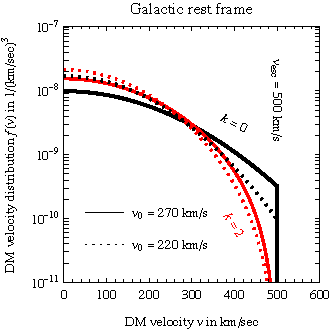
\includegraphics[width=0.45\textwidth]{figs/pVel}\qquad
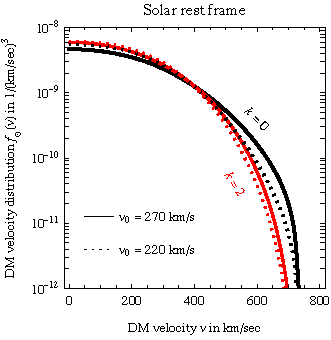
\includegraphics[width=0.44\textwidth]{figs/pVelsun}
$$
\caption[DM velocity distributions]{\em  \label{fig:DMv} {\bfseries DM velocity distributions}:  
the Maxwell-Boltzmann distribution 
with a sharp cutoff at $v=v_{\rm esc} = 500\,{\rm km/s}$ (thick black curve, $k=0$), 
and the distribution motivated by the $N$-body simulations, eq.~\eqref{eq:fk}, 
with a smooth cutoff computed for $k=2$ (red).
Two different values of $v_0$ are shown: $220~{\rm km/s}$ (dotted) and $270~{\rm km/s}$ (solid).
Left (right) panel shows the DM velocity distribution in the galactic (solar) rest frame (note
 the different scales on the horizontal and vertical axes in the two panels).
}
\end{figure}

\begin{figure}[!t]
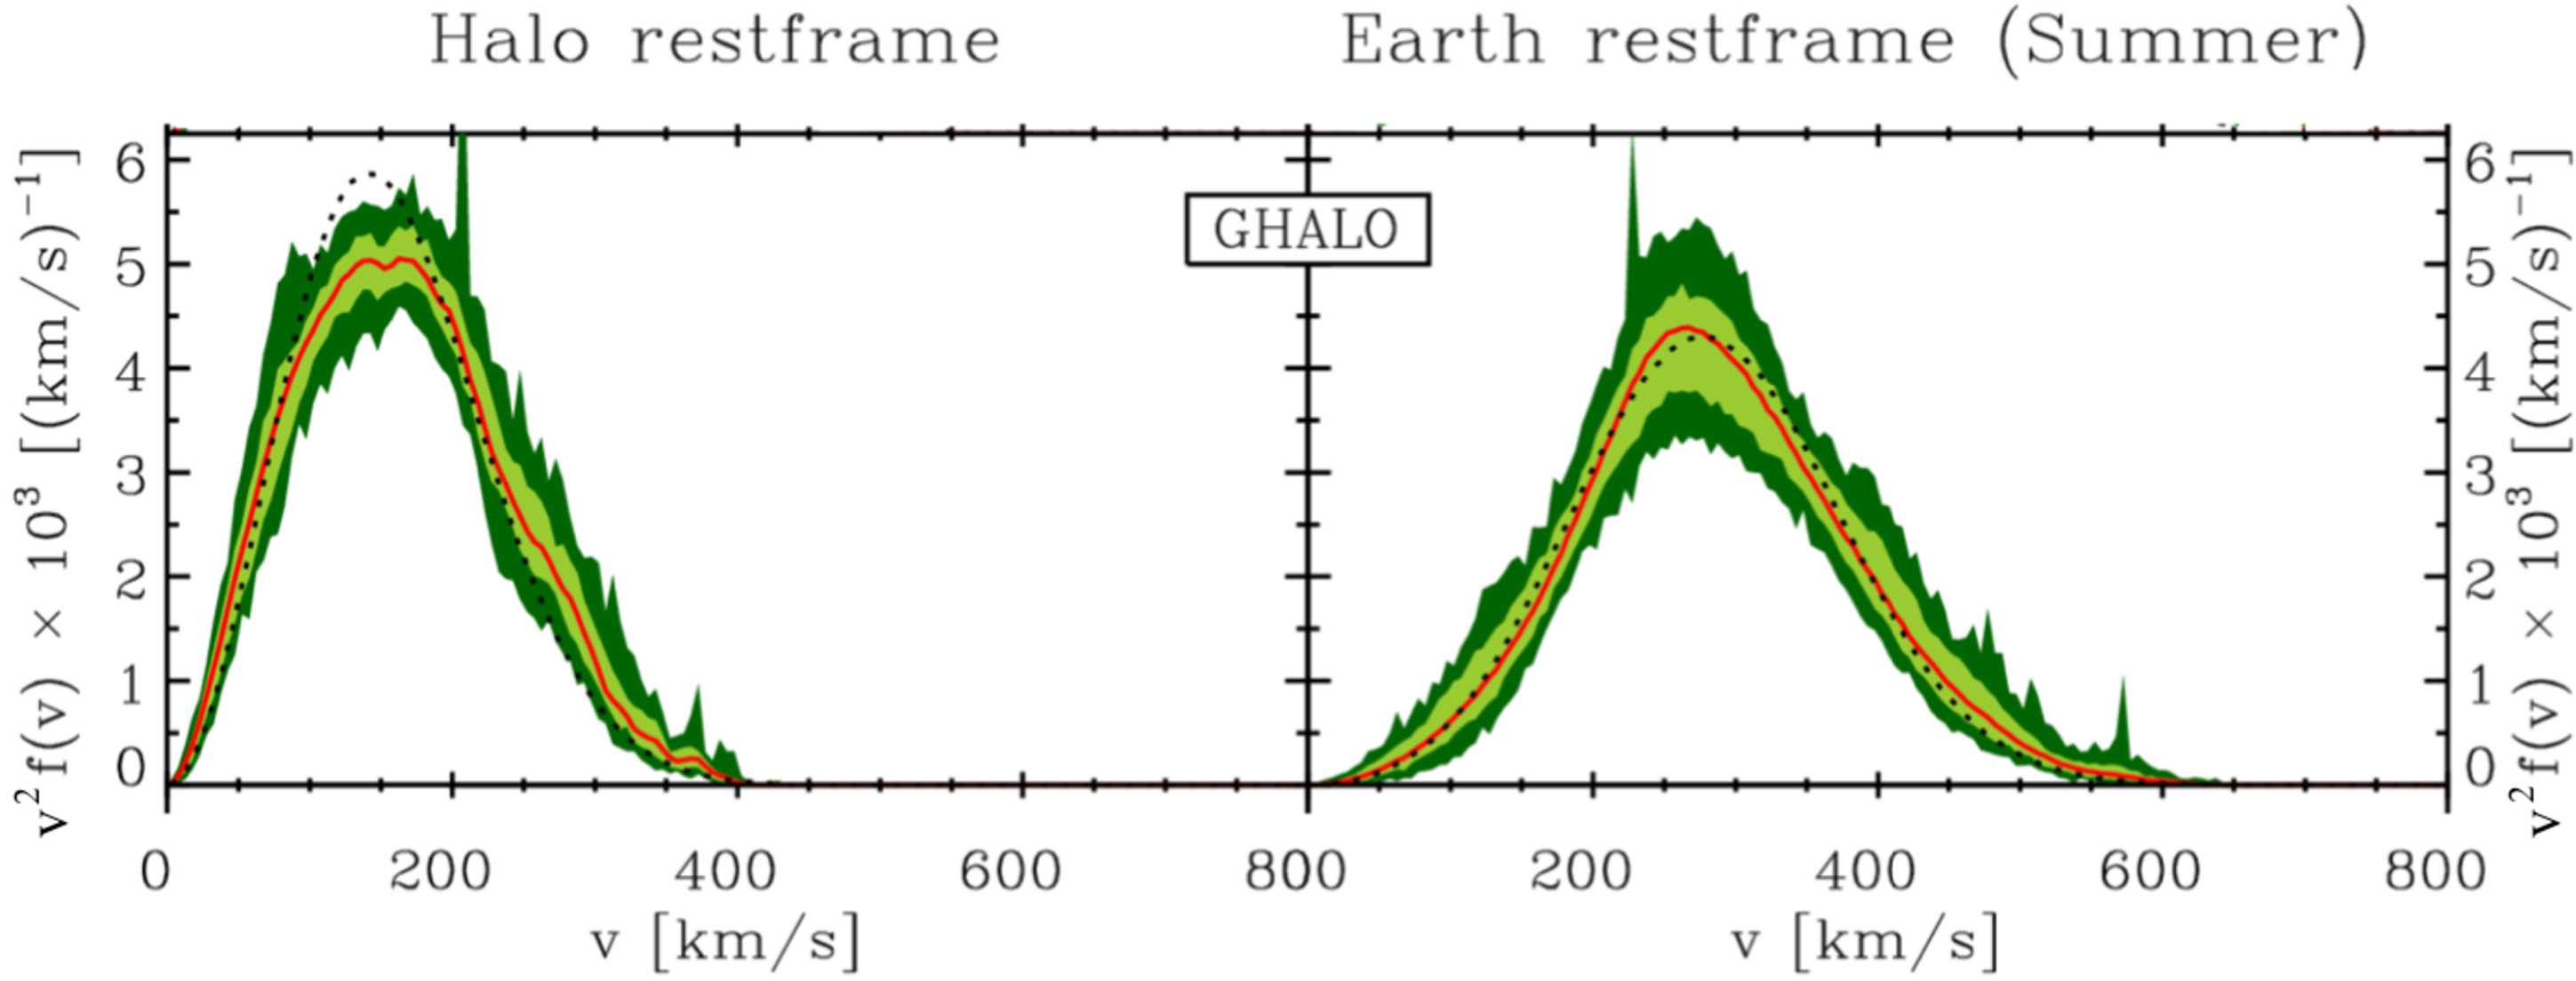
\includegraphics[width=\textwidth]{figs/velocity_distrib_Nbody}
\vspace{1cm}
\begin{minipage}{0.5\textwidth}
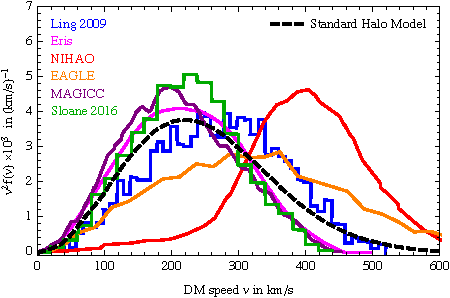
\includegraphics[width=\textwidth]{figs/velocity_distrib_hydro_mod}
\end{minipage}
\quad
\begin{minipage}{0.45\textwidth}
\centering
\caption[DM speed distributions from simulations]{\em \label{fig:vel:dep}
{\bfseries DM speed distributions from sample numerical simulations.} Top (adapted from \arxivref{0912.2358}{Kuhlen et al.~(2010)}~\cite{fvNbody}): distribution in the galactic rest frame (left) and in the Earth's rest frame  (right) as obtained from GHALO  $N$-body simulation. 
The solid red line is the average distribution, with the light (dark) green shaded regions giving the 68\% scatter (envelope). 
The dotted line is the best-fitting Maxwell-Boltzmann distribution.   
Left (adapted from \arxivref{1705.05853}{Bozorgnia and Bertone~(2017)}~\cite{fvNbody}): distribution in the galactic rest frame for a sample of hydrodynamical simulations. The dashed black line corresponds to the Maxwell-Boltzmann distribution with the peak speed of 220 km/s.}
\end{minipage}

\end{figure}



\section{Dark Matter velocity distribution}\label{sec:DMv}
\index{Velocity distribution}\index{DM abundance!velocity distribution}
Next, we turn our attention to the DM velocity distribution $f(\vec x, \vec v)$, where we will focus mostly on the Milky Way. The treatment can be easily extended to other galaxies, most notably to the dwarf galaxies, by replacing appropriately the parameters. Initially, we will neglect the dependance of DM velocity distribution on the position $\vec x$ (this is relaxed at the end of this section).
Furthermore, the DM velocity distribution in the galactic rest frame is almost always assumed to be isotropic, so that $f(v)$ is a function of $v = |\vec v|$ only, and we often speak of a DM {\em speed} distribution.

\smallskip

As discussed in section~\ref{sec:rho_from_analytic}, 
the Eddington formula relates a spherical density $\rho(r)$ to a spherical velocity distribution.
This was used to show in eq.\eq{isothermalsphere} that a Gaussian corresponds to an isothermal sphere $\rho \propto 1/r^2$.
The procedure can now be inverted to find a velocity distribution corresponding to the more realistic profiles discussed in section~\ref{rho(r)}.
For example, a power-law 
$\rho \propto 1/r^{\gamma}$ (appropriate at small $r$) 
corresponds to $f(v) \propto v^{(\gamma-6)/(2-\gamma)}$.
This provides an interesting approximation~\cite{AnalyticalHM} despite that
the assumptions behind the Eddington formula are not satisfied:
the distributions are not strictly time-independent, and baryonic matter forms non spherical disks.


\smallskip

This discussion suggests that the DM velocity distribution cannot exactly follow a Gaussian Maxwell-Boltzmann  distribution.
In particular, DM particles that happen to acquire a speed larger than the galactic escape velocity, $v_{\rm esc}$, tend to evaporate away.
To account for this, the DM  speed distribution in the galactic rest frame, $f(v)$, is often assumed to be an isotropic 
Maxwell-Boltzmann distribution that is sharply cut off at the finite escape speed
\begin{equation}
\label{eq:MB}
\bbox{f( v) = N\,  e^{-v^2/v_0^2} \ \Theta(v_{\rm esc}-v)}.
\end{equation}
The normalization constant is fixed such that $\int d^3v\, f(v) = 1$,
giving $N=\pi^{-3/2} v_0^{-3}$ in the limit $v_{\rm esc}\gg v_0$ (here $d^3v =4\pi v^2\, dv$). The parameters $v_{\rm esc}$ and $v_0$ are estimated as follows:
\begin{itemize}

\item[$\circ$] The virial theorem $\med{K} = -\frac12\med{V}$ 
applied to the isothermal sphere implies
$2\sigma^2 = \med{v^2}=v_{\rm circ}^2$ (see page \pageref{vcircisot})
where
$v_{\rm circ}$ is the local circular velocity, measured to be
$v_{\rm circ}\approx (220\pm 10)\km/\s$~\cite{astro-ph/9706293} from motions of the stars.
Since $\med{v^2}=3v_0^2/2$ this suggests $v_0 =\sqrt{2/3} \, v_{\rm circ}$. 
However, as discussed on page \pageref{vcircisot}, the approximation of an isothermal sphere for DM distribution is not entirely realistic. In particular, it implies 
an infinite escape velocity, since the enclosed mass $\Mcal (r)$ diverges for $r\to \infty$.


\item[$\circ$] Observations of stellar motions show that the local\footnote{That is, near the location of the solar system.} escape velocity from the Milky Way is~\cite{Smith:2006ym} 
\beq 
\label{eq:vesc:range}
\bbox{v_{\rm esc}\approx (544\pm 35)\km/\s}.
\eeq
Measured speeds of old stars, which are 
expected to have a speed distribution similar to DM~\cite{1704.04499}, 
suggest 
\beq \label{eq:rms:v0}
\bbox{220\,{\rm km/s}<v_0<270\,{\rm  km/s}}.
\eeq




\listpart{$N$-body simulations indicate a more complex picture \cite{fvNbody}.\index{Numerical simulations!speed distribution}}

\item[$\circ$] 
$N$-body simulations seem to suggest a distribution with bumps and dips, deviating significantly from a simple Maxwell-Boltzmann (see fig.~\ref{fig:vel:dep}). Furthermore, the distribution features a smoother cut-off at $v<v_{\rm esc}$ and can be parameterised as (\arxivref{1010.4300}{Lisanti et al.~(2011)}, \arxivref{0912.2358}{Kuhlen et al.~(2010)} \cite{fvNbody})
\begin{equation}
\label{eq:fk}
\bbox{ f(v)= N_k \left[\exp\left(\frac{v_{\rm esc}^2-v^2}{kv_0^2}\right)-1\right]^k  \Theta(v_{\rm esc}-v)},
\end{equation}
with $1.5<k<3.5$. The Maxwell-Boltzmann 
distribution of eq.~\eqref{eq:MB} is obtained in the limit $k\rightarrow 0$.
These velocity distributions are plotted in fig.\fig{DMv}a.

\item[$\circ$] 
More recent hydrodynamical simulations, which include baryons, seem 
to suggest instead a speed distribution closer to the standard Maxwell-Boltzmann, albeit with a $v_0$ that is  by a few tens of km/s larger than the one in eq.~(\ref{eq:rms:v0}). 
The spread among different simulations, as well as among different realizations of a single simulation is so large though, that a more precise determination of $v_0$ does not seem to be possible. Hydrodynamical simulations also seem to find a more isotropic distribution than the DM-only ones.
\end{itemize}

\begin{figure}[!t]
\begin{minipage}{0.55\textwidth}
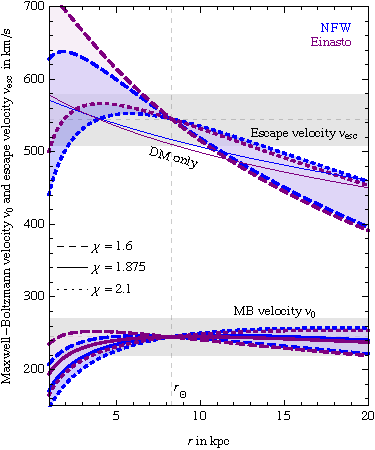
\includegraphics[width=\textwidth]{figs/plotv0vesc}
\end{minipage}
\quad
\begin{minipage}{0.40\textwidth}
\caption[DM speeds a s a function of the position in the Galaxy]{\em  \label{fig:v0andvescofr} {\bfseries Illustration of the dependence of DM speeds on the position in the Galaxy}: the Maxwell-Boltzmann parameter $v_0$ in the bottom, and the escape velocity $v_{\rm esc}$ in the top of the plot, according to the relations (\ref{eq:pseudospacedensity}) and (\ref{eq:vescofr}). The blue (purple) lines are for NFW (Einasto) DM profiles. The solid lines are for Bertschinger's $\chi = 1.875$, and dashed (dotted) lines for $\chi=1.6(2.1)$. 
The normalizations are such that at the solar position $r_\odot$ the $v_0$ and $v_{\rm esc}$ coincide with the central values in eq.s~(\ref{eq:rms:v0}) and~(\ref{eq:vesc:range}), respectively, while the grey horizontal bands illustrate the plausible uncertainty ranges on these values. 
The thin solid lines  in the upper part of the plot denote $v_{\rm esc}(r)$ for a galaxy containing only DM.}
\end{minipage}
\end{figure}


The average DM speed varies with the position $r$ in the Galaxy \cite{fvofr}, see figure \ref{fig:v0andvescofr}. Numerical simulations suggest a simple power law scaling 
\beq
v^3_0(r) \propto r^\chi \rho(r),
\label{eq:pseudospacedensity}
\eeq
with the exponent $\chi \approx 1.9 - 2.1$ in the DM-only simulations,
 and $\chi \approx 1.60 - 1.67$ in the simulations that include baryons. 
 In fact, already the pioneering work Bertschinger (1985)~\cite{fvofr} predicted such a relation, with $\chi \approx 1.875$, based on spherically symmetric collapse.\footnote{The formalism in Bertschinger (1985) is somewhat different from the one adopted here; see Taylor and Navarro (2001) for the recast. 
 The ratio $ \rho/v_0^3$ is called the (pseudo-)phase-space density.}
 The size of positional variation in $v_0$  depends on the assumed values of $\chi$ and the DM density profile $\rho(r)$, see eq.~\eqref{eq:pseudospacedensity}. In practice, however, 
 $v_0$ does not change much, at least for $r$ within a few kpc of the location of the Sun, $r_\odot\simeq 8.3$\,kpc.
 For the $\chi$ values obtained from the DM-only simulations, DM particles are on average slower in the center of the Galaxy, and  faster on the outskirts,  for $r$ beyond the position of the solar system.
 For the $\chi$ values that follow from the simulations that include baryons, on the other hand, the opposite tendency is found.
The relation (\ref{eq:pseudospacedensity}) holds over 2.5 orders of magnitude in $r$, from roughly $r \approx 0.1$ kpc (the resolution limit of the $N$-body simulations) up to at least $r \approx 20$ kpc. 
 
The escape velocity $v_{\rm esc}$
is also clearly position dependent. If one were to take just the DM into account, the escape velocity would have been straightforwardly predicted from its gravitational potential, which is determined by the DM mass enclosed within radius $r$. In the inner part of the Galaxy, though, the baryons constitute a significant fraction of matter content, which then makes the determination of $v_{\rm esc}(r)$ more involved. The following empirical parametrization is sometimes used (see \arxivref{1005.1779}{Cirelli and Cline (2010)} in \cite{fvofr}):
\beq
\label{eq:vescofr}
v_{\rm esc}^2(r) = 2 v_0^2(r) \Big[2.29 + \ln(10 \, {\rm kpc}/r) \Big].
\eeq
Using eq.~(\ref{eq:pseudospacedensity}) for $v_0(r)$, one can find that the escape velocity is typically highest in the inner galaxy, as expected, although the detailed behavior depends on the values of $\chi$ and $\rho$.

\smallskip

Extra possible complications, such as DM streams, will be discussed in section~\ref{sec:DMstreams}.
Note that, while DM velocity distribution is rather uncertain, it is robust that the bulk of DM has $v \sim 10^{-3}$, and for many predictions this is good enough and the details are not so important. In other cases, these details matter and uncertainties on predictions can be very large. 
Among the many uncertainties, it is worth mentioning that
extra DM particles with large speeds around $v_{\rm esc}$ could be 
present, if the Milky Way recently accreted extra DM, or even with speeds well above  $v_{\rm esc}$, if DM is being boosted by interactions with cosmic rays (see section \ref{BoostedDM}).




\setstretch{0.98}
\subsection{DM velocity with respect to the Sun}\label{sec:DMvsun}\label{Velocity distribution!with respect to the Sun}
The previous subsection mostly dealt with DM velocity (or speed) distribution in the rest frame of the Galaxy.\footnote{Our galaxy and the DM that it contains move at about 600 km/s with respect to the CMB rest frame. This movement, however, does not affect our relative velocity with respect to DM in the Galaxy and is therefore of little interest.} 
Of more immediate phenomenological interest, however, is the DM velocity distribution in the solar local frame, $f_\odot(\vec v)$. The $f_\odot(\vec v)$ distribution, for instance, enters the estimates of  DM capture by the Sun, and the subsequent neutrino flux (see section~\ref{sec:captureDMsun}).
The $f_\odot(\vec v)$ is straightforwardly obtained from the velocity distribution in the galactic frame, $f(\vec v)$, by performing a Galilean transformation
$f_\odot(\vec v) = f(\vec v+ \vec v_\odot)$
where
\beq
\label{eq:vodot}
\vec v_\odot = (0,220,0) \km/{\rm s} + (10,13,7) \km/{\rm s},
\eeq
is the velocity of the Sun, here written as the sum of the local Galactic rotational velocity, and the Sun's peculiar velocity.
We used Galactic coordinates, where $\hat{\mb{x}}$ points from the Sun toward the Galactic center, $\hat{\mb{y}}$ in the direction of disk rotation, and $\hat{\mb{z}}$ toward the galactic north pole.
The modulus of $\vec v_\odot$ is $v_\odot \approx 233\,\km/\sec$.


Below, we will also need the spherical angular average of $f_\odot$, which is given by
\begin{equation}
\label{eq:fsunav}
f_\odot(v) =  \frac{1}{2} \int_{-1}^{+1} d\cos\theta  ~f\left(\sqrt{v^2 + v_\odot^2 + 2 v v_\odot \cos\theta}\right).
\end{equation}
The numerical results for several examples of $f_\odot(v)$ are plotted in fig.\fig{DMv}b.


\begin{figure}[t]
\begin{center}
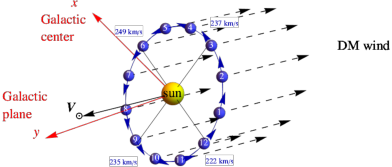
\includegraphics[width=0.64\textwidth]{figs/DDmodulationEarth}
\end{center}
\caption[DM wind]{\em The solar system and the Earth (blue spheres at indicated months)
are moving through the stationary DM halo, 
which results in the effective `{\bfseries DM wind}' in the Earth's frame. 
The DM wind is at the maximal speed, around $v_\oplus\approx 249\,{\rm km/s}$, 
at the beginning of June, when the Earth is moving fastest in the direction of the galactic disk's rotation, 
and at the minimal speed at the beginning of December, when the Earth  is moving fastest in the opposite direction to the galactic disk's rotation. 
}
\label{fig:DMwind}
\end{figure}

%\setstretch{1}


\subsection{DM velocity with respect to the Earth}\label{sec:DM:velocity:Earth}\label{Velocity distribution!with respect to the Earth}
The DM velocity distribution in the Earth's rest frame, $f_\oplus(v,t)$, is obtained in terms of the velocity distribution in the galactic frame, $ f(\vec v)$, through
\begin{equation}
\label{eq:fearth}
f_\oplus(\vec v,t) = f(\vec v+\vec v_\oplus(t))\,.
\end{equation}
Here $\vec v_\oplus(t)$ is the relative motion of the Earth with respect to the galactic frame.
It is given by
\beq \vec v_\oplus(t) = \vec v_\odot + V_\oplus \bigg[ \hat{\mb{\varepsilon}}_1 \cos\omega(t-t_1) + \hat{\mb{\varepsilon}}_2 \sin \omega(t-t_1)\bigg],
\eeq
where
$\vec v_\odot $ is the velocity of the Sun,
$V_\oplus = 29.8\km/\sec$ is the Earth's orbital speed, $\omega=2\pi/\yr$,
$t_1 = 0.218\,{\rm yr} = $ March 21 is the time of the
spring equinox, while
$ \hat{\mb{\varepsilon}}_1 $ and $ \hat{\mb{\varepsilon}}_2$ are the orthogonal unit vectors tangent to Earth's orbit 
 at spring equinox and summer solstice
(at $t_1 + \yr/4$), respectively.
In Galactic coordinates (defined in section~\ref{sec:DMvsun}, eq. \eqref{eq:vodot}) one has
\beq
\hat{\mb{\varepsilon}}_1 = (\phantom{-}0.9931,\,0.1170,\,-0.0103),\qquad
\hat{\mb{\varepsilon}}_2= (-0.0670,\,0.4927,\,-0.8676).
\eeq
Consequently, the modulus of the Earth's velocity is
\beq 
\label{eq:voplus:time}
v_\oplus(t) = \sqrt{v_\odot^2+ V_\oplus^2 + 2b v_\odot V_\oplus\cos[\omega(t-t_c)]}
\simeq
v_\odot + \frac{V_\oplus^2}{2v_\odot}+b V_\oplus \cos[\omega(t-t_c)],
\eeq
where
\beq b = \frac{\sqrt{(\hat{\mb{\varepsilon}}_1\cdot \vec v_\odot)^2+(\hat{\mb{\varepsilon}}_2\cdot \vec v_\odot)^2}}{ v_\odot},
\approx 0.490\eeq
is the sine of the angle between $\vec v_\odot$ and the normal to the orbital plane of the Earth,
and
\beq
t_c=t_1 + \frac{1}{\omega}\arctan\frac{\hat{\mb{\varepsilon}}_2\cdot \vec v_\odot}{\hat{\mb{\varepsilon}}_1\cdot \vec v_\odot}\approx0.415\yr=\hbox{June 2},
\eeq
is the time at which $v_\oplus(t)$ is maximal, $v_\oplus(t_1) \approx 249\km/\sec$.
The minimal Earth's velocity is $v_\oplus(t_1 + \yr/2)\approx 222\km/\sec$.
The geometry of different contributions to $v_\oplus(t) $  is plotted in fig.\fig{DMwind}.
The time variation of $v_\oplus(t)$ has phenomenological consequences: it leads to the annual modulation of DM direct detection signals, as discussed in section~\ref{DMmodulation}.



\section{Beyond the dark spherical (and isotropic) cow limit}\label{sec:asphericalcow}
To a first approximation the present day DM halos, at least the galactic ones, 
are often assumed by particle physicists to be spherically symmetric, static (therefore also in a steady state), homogeneous,
and filled with particles obeying an isotropic velocity distribution. 
However, as we have encountered repeatedly above, this is just an approximation. 
A more detailed analysis shows that significant deviations from this picture can occur.
We already discussed one important example: the expected presence of {\bf subhalos}, i.e.,~clumps of DM (see section~\ref{sec:resNbody}).
Other deviations, discussed in this section, include departures from sphericity, from the assumption of static (and more generally, steady state) DM distributions, from the isotropy of DM velocities, etc.  
These deviations are not only relevant per se, since they are an essential stepping stone toward our understanding of the astrophysics of DM and how the microscopic properties of DM affect its distribution, but can also impact significantly the predicted signals in direct or indirect detection, see chapters \ref{chapter:direct} and \ref{chapter:indirect}.
 

\subsection{Non-sphericity of DM halos}\label{sec:nonSphericalHalo} \index{DM abundance!asphericity}
Numerical simulations\index{Numerical simulations!halo shapes} consistently find DM halos with an ellipsoidal shape~\cite{haloshape}.\footnote{An ellipsoid is characterized by three semi-axes $a$, $b$ and $c$, with $a \ge b \ge c$ by convention. It is {\em prolate} (rugby ball shaped) if $a > b \approx c$, {\em oblate} (pancake shaped) if $a \approx b > c$, and {\em triaxial} otherwise. In terms of the triaxiality parameter $T \equiv (a^2-b^2)/(a^2-c^2)$ prolate means $T > 2/3$, oblate $T < 1/3$, and triaxial $1/3 < T < 2/3$.} 
While the details can be complex (for one, it is not trivial to define the iso-density surfaces that identify the ellipsoid and its inner layers) and somewhat simulation-dependent, there seems to be consensus on a few general results. i) Galactic DM halos (and possibly also cluster halos) are triaxial, with a tendency towards prolate. Typical axes ratios are $b/a \sim 0.65$ and $c/b \sim 0.8$.
The shape can vary mildly  with the distance from the center: a halo can be thought of as a deformed-onion-like system with the inner shells  typically more prolate, while the outer shells  are progressively rounder; the shells are rather well aligned. ii) More massive halos are more triaxial. iii) The addition of baryons makes the halos rounder and more oblate. iv) The detailed dynamical mechanisms by which the triaxial shapes are achieved are still under study. They are probably related to the history of formation of the halos within a complex network of DM structures: the prolate direction might be a remnant of the incoming direction of DM particles from filaments, while the more isotropic accretion of late periods can result in rounder forms. In this sense, the shape of a halo can evolve as a function of time and redshift.\\
The results of observations via weak lensing of stacked galactic and cluster halos show some evidence for triaxiality too. For the specific case of the Milky Way, however, the situation is more confusing. One would normally expect for the Milky Way halo to be triaxial, with ratios of axes similar to those quoted above. However, the attempted measurements, using in particular the observations of stellar streams such as the Sagittarius stream or of stellar kinematics (notably from the {\sc Gaia} mission), have resulted in indications of a halo that is anything from prolate to oblate to spherical. 

\subsection{Rotating DM halos} \label{sec:halocorotation} \index{DM abundance!rotating halos}
The issue of spinning DM halos, in particular those that surround the rotating disks of spiral galaxies, is intrinsically connected with the formation of the disks themselves, which is an active research field in astrophysics~\cite{books_galaxy_formation,corotation}. The standard story is the one we have already alluded to in the beginning of this chapter, and goes roughly as follows. Initially, in the early stages of structure formation, both DM and baryonic gas were in the form of diffuse, roundish clouds. These clouds gained an initial non-vanishing angular momentum as a consequence of the torques applied by the tidal gravitational fields from neighbouring over-densities (a mechanism that goes under the name of Tidal Torque Theory). Subsequently, the baryonic gas, which is dissipational, i.e.,~it can radiate away electromagnetically part of its energy, started to cool and sink to the center. Barring significant inflows and outflows, it can be assumed that its angular momentum was conserved during the cooling. This means that the baryonic gas cannot collapse all the way to the center, but instead re-arranges itself into a rotationally supported spinning disk.  
DM particles, on the contrary, cannot dissipate energy (see page~\pageref{dissipationless}). DM clouds therefore shrunk in size,\footnote{Remember from section~\ref{sec:rho_from_analytic} that the virial theorem predicts the final halo radius to be 1/2 of the `turnaround radius'.} which somewhat increased their rotational velocities, but the collapse came to a halt as soon as the systems virialized.
As a result, the initial large and slowly spinning clouds morphed into the familiar configurations of a small rapidly rotating galactic disk surrounded by a much larger DM halo whose spin has not increased significantly. It is in this sense that the approximation of a static DM halo can be quite adequate.

The somewhat na\"ive picture above is essentially supported by the results of numerical simulations.\index{Numerical simulations!halo rotation} The simulations also confirm that, as expected, the rotation axes of the disks and their host DM halos are roughly aligned, within at most 30$^\circ$ or so (`co-rotating DM halo'). The picture can be made more complex by several `environmental' phenomena intervening at different stages of galaxy formation (cold inflows of baryonic gas depositing angular momentum in the forming disk, halos merging, satellite galaxy accretion,\ldots) and/or by baryonic physics.

\smallskip

For a more quantitative treatment one can introduce the dimensionless {\em spin parameter} $\lambda$, which for any object such as a DM halo or a galactic disk is defined as $\lambda = j_{\rm sp}\  E^{1/2}_{\rm tot}/  G \, \Mcal ^{3/2}_{\rm tot}$. Here, $j_{\rm sp}$ is the {\em specific} angular momentum, i.e.,~the total angular momentum of the system divided by its mass: 
$j_{\rm sp} = |\vec{J}|/\Mcal_{\rm tot}$, 
where $\mb{J}$ is the total angular momentum,\footnote{Angular momentum is defined as $\vec{J} = \Sigma_{i}  \vec{r_i} \times m_i\vec{v_i}$, where the sum runs over all the elements  of the system, e.g.,~DM `particles' or individual stars. The elements have masses $m_i$,  are at positions $\vec r_i$ as measured from the system's center,  and have velocities $\vec v_i$ in the center of mass system. 
} 
$E_{\rm tot}$ is the absolute value of the total energy  of the system (sum of kinetic and potential energy -- note that this sum is negative), and $\Mcal _{\rm tot}$ its total mass. 
The parameter $\lambda$ essentially measures the fraction of the total energy of the system that is stored in its spinning motion. It allows to compare consistently systems of different masses and sizes. For an isolated system undergoing gravitational dissipation-less evolution, such as the DM halo, $\lambda$ is conserved, since all the quantities entering its definition are conserved.
Simulations consistently find $\lambda$ to be distributed around $\lambda_{\rm DM \ halo} \approx 0.04$, in agreement with theoretical expectations. 
In contrast, for a dissipational system such as the baryonic gas, $E_{\rm tot}$ increases since the binding energy increases when the cloud shrinks to form the disk. 
One finds $\lambda_{\rm disk} \approx 0.4$ at the end of the evolution. 
The result $\lambda_{\rm disk} \gg \lambda_{\rm DM \ halo} \neq 0$ expresses in formul\ae{} that the rotation of the DM halo exists, but plays only a minor role.
 

The impact of bulk DM halo co-rotation (or even counter-rotation\footnote{A counter-rotating configuration can occur when massive inflows cause the baryonic disk to flip in the late stages of galaxy formation, something which is observed, albeit rarely, in simulations.}) on direct detection signals has been phenomenologically investigated in a few works~\cite{corotation}. These found  rather modest modifications of DM scattering rates, and thus also rather small changes in the derived bounds on the scattering cross sections (see chapter \ref{chapter:direct}),  from about 10\% up to a factor ${\mathcal O}(2)$ in the extreme cases. 

\subsection{Dark disk?} \label{sec:darkdisk} \index{DM abundance!dark disk}\index{Dark!disk}
Some numerical simulations find in their Milky Way-like simulated galaxies disks of Dark Matter that are aligned with the stellar disks~\cite{darkdisk}. Dark disks seem to be created by  the disruption and dragging of DM satellites as well as simply through the gravitational pull of the baryonic disk. Their contribution to the local DM density varies between a few percent and 1.5 times the estimate for $\rho_\odot$ in \eqref{eq:rhosun:value}, depending on the simulation. The disk is found in some cases to be dragged by the baryonic one and thus co-rotating, with a low lag speed of about 50 km/s. 
In other simulations, however, the dark disks are observed only very rarely, from which one would deduce that dark disks are unlikely to be relevant.

How likely it is for the dark disks to form also depends on the microscopic properties of DM. 
Some theoretical works speculated that a small fraction of Dark Matter (up to 5\%) could consist of a dissipational and/or partially self-interacting substance that can therefore collapse and form a thin dark disk, parallel to the galactic disk~\cite{darkdisk}. 
This theoretical possibility was dubbed Double Disk Dark Matter (DDDM).
If present, a dark disk would have an impact on DM direct and indirect detection. For instance, it would lead to enhanced rates for capture of DM particles inside the Sun and Earth (especially in the case of co-rotation, because low relative velocities make the capture easier), and therefore possibly to enhanced neutrino fluxes (see section~\ref{sec:DMnu}).
A more speculative effect on comet impacts and dinosaur extinction is mentioned in section~\ref{sec:anomanom}.

Recent data from the {\sc Gaia} mission indicate, however, that at most $1\%$ of DM can be in the form of a thin dark disk~\cite{darkdisk}. 


\subsection{Anisotropic DM velocity distribution}\label{sec:anisotropicvelocity}
 $N$-body simulations show that the orbits taken by dark matter particles are  preferentially radial, resulting in an anisotropic velocity distribution~\cite{anisotropicvelocity}. 
Such a velocity anisotropy is not surprising for non-spherical halos, but it can also arise in halos exhibiting a spherically symmetric density profile.

More concretely, numerical simulations indicate that the radial velocity $v_r$ and the tangential velocity $v_t = \sqrt{v_\theta^2 + v_\phi^2}$
follow different profiles, approximated by non-Maxwellian distributions of the form
\beq 
f(v_r, r) \approx N_r \exp\left[-\left(\frac{v^2_r}{v_{0r}^2(r)}\right)^{\alpha_r(r)} \right],\qquad
 f(v_t, r)\approx N_t v_t  \exp\left[-\left(\frac{v^2_t}{v_{0t}^2(r)}\right)^{\alpha_t(r)} \right],
\eeq
where $N_r$ and $N_t$ are the appropriate normalization factors determined as in eq.~(\ref{eq:MB}).
Writing $v_{0r}= \beta_r(r) \, v_{\rm circ}(r)$ 
and  $v_{0t}= \beta_t(r) \, v_{\rm circ}(r)$, the simulations suggest that at the position of the solar system~\cite{fvNbody} 
\beq 
\alpha_r \sim 1, \qquad \beta_r \sim 0.7, \qquad
\alpha_t \sim0.7, \qquad \beta_t \sim 0.4,
\eeq
implying $v_{0t}  \sim 120 \km/\sec$, smaller than 
$v_{0r}\sim 200 \km/\s$.
All four parameters, $ \alpha_r,\alpha_t,\beta_r,\beta_t$, become smaller at smaller $r$, in agreement with the discussion in section \ref{sec:DMv} for the case of DM only simulations. 
The velocity anisotropy parameter, 
\beq
\label{eq:vanisotropyparam}
\beta_{\rm anis} \equiv 1-\frac{v^2_{0t}}{v^2_{0r}},
\eeq
equals 
$\beta_{\rm anis} = 1$ in the limit  where DM particles are all on radial orbits;
$\beta_{\rm anis}=-\infty$ for all tangential orbits;
while the isotropic case corresponds to $\beta_{\rm anis} = 0$. 
In general, $\beta_{\rm anis}$ can vary as a function of $r$: the
simulations find $\beta_{\rm anis} \approx 0$ in the central regions of galactic halos, and $\beta_{\rm anis} \approx 0.5$ in the outer regions.



\subsection{DM streams}\label{sec:DMstreams}  \index{DM abundance!streams}
Galaxy formation is a continuous process: our galaxy is tidally stripping the smaller neighbouring galaxies and accreting mass to the expense of these smaller galaxies. Most probably, it is also tidally stripping and digesting its own DM subhalos close to the galactic center. These phenomena create streams of DM transpiercing the galaxy in various directions~\cite{streams}. Some of these (such as the Sagittarius stream) were observationally identified thanks to the accompanying stellar flow. However, the numerical simulations predict the existence of many more DM streams.
  
DM streams are unlikely to contribute significantly to the local DM density: simulations find that they typically contain between 0.1\% and 1\% of the smooth average density of the underlying halo. However, they are directional and cold (i.e.,~characterized by low velocity dispersion). Therefore, they can modify significantly the DM velocity distribution from the one quoted in eq.~(\ref{eq:MB}) or in eq.~(\ref{eq:fk}) to $f_{\rm halo + str}(\vec v) =  (1-\rho_{\rm str} / \rho_\odot) f(\vec v,v_0) + \left( \rho_{\rm str}/\rho_\odot \right) f_{\rm str}(\vec v_{\rm str})$. Here, $\rho_{\rm str}$ and $\vec v_{\rm str}$ are respectively the local DM density and velocity of the stream, and $f_{\rm str}$ is the functional form of the velocity distribution in the stream, which can be Maxwell-Boltzmann or not. 
Furthermore, one expects a small density $\sim 10^{-2-5}\GeV/\cm^3$ of extra DM particles trapped
in the Local Group and in the Virgo Supercluster to cross the Milky Way with higher velocities $\sim 600-1000\,{\rm km/s}$. 
Such an addition can be significant in the high-speed tail of the DM velocity distribution, possibly leading to important effects in DM direct detection. 

\medskip

It has also been argued that the DM galactic halos should exhibit {\bf caustics}, i.e.,~accumulation surfaces of very high density, corresponding to the turnaround points for particles moving on gravitationally bound orbits (technically, the density is even divergent, in the limit of vanishing velocity dispersion)~\cite{caustics}.\index{DM abundance!caustics} 
Caustics are expected to be a generic phenomenon in cold and collisionless fluids like DM, i.e.,~fluids with negligible velocity dispersion and negligible internal interactions. 
They would materialize as rings of enhanced density at specific radii in the inner and outer regions of the galaxy. 
Some evidence has been claimed for their existence in the Milky Way and in other galaxies, based on peculiar over-densities and regularly spaced bumps in the rotation curves~\cite{caustics}.



\subsection{DM around black holes}\label{sec:DMBH}\index{DM abundance!around black holes}
A higher DM density is expected to accumulate around black holes, 
which are known to exist with masses from few $M_\odot$ (stellar BH) to $10^{10}\, M_\odot$ (supermassive BH at the center of galaxies), including intermediate mass black holes (IMBH) with typical masses $10^2-10^5\, M_\odot$.
The accumulation is usually described by defining the radius of gravitational influence $r_{\rm in}$ of the black hole
as the radius within which the enclosed DM mass is twice the BH mass.
Simulations suggest that a `spiked' DM density profile starts inside $r_{\rm sp}\approx 0.2\, r_{\rm in}$ with power-law form~\cite{DMBH}
\beq \label{eq:DMspike} \frac{\rho_{\rm DM}(r)}{\rho_{\rm DM}(r_{\rm sp})}\approx  
\left\{\begin{array}{ll}
(r_{\rm sp}/r)^{\gamma_{\rm sp}} & \hbox{at $r<r_{\rm sp}$},\\
(r_{\rm sp}/r)^{\gamma}  & \hbox{at $r>r_{\rm sp}$},
\end{array}\right.
\eeq
where $\gamma_{\rm sp}\approx 1.5-2.5$, or perhaps
$\gamma_{\rm sp}= (9-2\gamma)/(4-\gamma)$ assuming adiabatic growth (\arxivref{astro-ph/9906391}{Gondolo and Silk} in~\cite{DMBH}).
Here $\gamma$ is the slope of the DM density profile ignoring the BH,
for example $\gamma=1$ for a BH located in the center of a galaxy with the NFW DM profile, as discussed in section~\ref{rho(r)}.
DM spikes can be softened or disrupted by stellar heating, galaxy mergers, etc.

If such DM spikes exist, they would make black holes good targets for DM indirect detection. Several groups have considered this possibility, in particular around the SMBH in the center of galaxies \cite{DMBH}, around IMBH \cite{DMIMBH} and around PBH (see in this case the discussion in section \ref{sec:PBHs}).
\arxivref{2212.05664}{Chan and Lee (2023)} and \arxivref{2402.03751}{(2024)} in~\cite{DynamicalFriction} claim indirect evidence for such DM spikes based on DM friction (section~\ref{sec:DynamicalFriction}).




\section{Dynamical friction}\label{sec:DynamicalFriction}\index{Dynamical friction}
We end this chapter with a short discussion of the effect of the diffuse DM density on the motion of celestial bodies.
The DM corpuscules exert a tiny but non-negligible gravitational force on bodies such as planets, stars and black holes.
As realized by Chandrasekhar, this has a non-trivial consequence:
a  massive body moving with a certain speed with respect to ambient DM experiences a gravitational friction force known as {\em dynamical friction}~\cite{DynamicalFriction} (this is in addition to the possible aerodynamical friction due to particle interactions).

The phenomenon can be qualitatively understood as follows:
as the massive body plows through ambient matter, it attracts the ambient particles and they accumulate in its wake; this creates an over-density and thus a gravitational force that pulls the body back with respect to its direction of motion.
Dynamical friction is sourced also by ordinary matter (e.g.~diffuse interstellar gas), and it has the effect that stars tend to sink towards the galactic center, and planets toward their stars.
Although ordinary matter is denser than dark matter in many environments, our focus in this discussion is on the DM-induced dynamical friction.

To provide a rough estimate of the effect, consider DM initially at rest at a distance $r$ from a body with mass ${\cal M}$ which is moving with speed $V$.
DM falls onto the massive body 
in a free-fall time, $\Delta t\sim (r^3/G{\cal M})^{1/2}$.
During the time interval $\Delta t$ the body attracts a mass $\Delta {\cal M} \sim  r^3 \rho_{\rm DM}  \sim G {\cal M}\rho\Delta t^2$, where $\rho_{\rm DM}$ is the DM density,
and travels a distance $\Delta x = V\Delta t$. The consequent gravitational force
is $F_{\rm DM} \sim -G {\cal M}\,\Delta {\cal M}/\Delta x^2 \sim -G^2 {\cal M}^2 \rho_{\rm DM}/V^2$.


More precisely, assuming that DM has a velocity distribution $f(v)$, and that it is made of bodies much lighter than ${\cal M}$, its dynamical friction is given by
\beq \label{eq:df}
\bbox{\vec{F}_{\rm DM} = -4\pi G^2{\cal M}^2  \rho_{\rm DM}  \frac{\vec{V}}{V^3}\ell \wp}~,
\eeq
where $\ell \sim 10$ is an infra-red enhancement due to the long-range nature of gravity
and $\wp \le 1$ is the fraction of DM particles slower than $V$, 
\beq \wp = \int_0^V 4\pi v^2\, dv \, f(v) = {\rm erf}\frac{V}{v_0} - \frac{2V}{\sqrt{\pi} v_0} e^{-V^2/v_0^2},\qquad
\hbox{for $f(v)\propto e^{-v^2/v_0^2}$, as in eq.\eq{MB}}.\eeq
The consequent energy loss is 
\beq \label{eq:WDMdynf}
W_{\rm DM} = \vec{F}_{\rm DM}\cdot\vec{V} = -4\pi G^2 \rho_{\rm DM} {\cal M}^2\wp \ell/V.\eeq

\medskip

Dynamical friction is a purely gravitational effect that allows, in principle, to probe 
the very existence of DM (some authors challenge it claiming that its dynamical friction effect is not observed, see section~\ref{sec:cuspcore}), as well as its density and its velocity distribution.\index{Gravitational waves as a probe of DM}

Concerning probing the DM density, binary systems are particularly suitable: DM is denser and the energy loss due to its dynamical friction can compete with the energy loss due to the emission of gravitational waves,
affecting the observable phase and/or the frequency spectrum (see section \ref{sec:NANOgrav}).
Constraints on DM density have been derived from various sources:
from binary pulsars ($\rho_{\rm DM}\circa{<} 10^5\GeV/\cm^3$), 
from binary solar-mass black holes (two anomalies are interpreted as a possible observation
of DM with $\rho_{\rm DM} \sim 10^{11-13}\GeV/\cm^3$), and from
super-massive black holes~\cite{DynamicalFriction}.



